\documentclass[a4paper, oneside]{memoir}% Document class
\usepackage[a4paper]{geometry}			% Margins
\usepackage{lmodern}
\usepackage{graphicx}
\usepackage{float}
\usepackage{listings}
\usepackage[small,compact]{titlesec}	% No 'chapter' in chapter headings.
\graphicspath{{Media/}}					% Directory that holds images.

\titleformat{\chapter}[hang]
{\normalfont\Large\bfseries}{\thechapter}{1em}{\Large}
\titlespacing{\chapter}{0pt}{*0}{*1}

\titleformat{\chapter}{\Huge\bfseries}{\thechapter}{1em}{}
\titleformat{\section}{\LARGE\bfseries}{\thesection}{1em}{}
\titleformat{\subsection}{\Large\bfseries}{\thesubsection}{1em}{}
\titleformat{\subsubsection}{\normalsize\bfseries}{\thesubsubsection}{1em}{}

\usepackage[disable]{todonotes}					% Todo Notes
\usepackage[draft]{fixme}
\newcommand{\bycykelwithoutspace}{Aalborg Bycykel}
\newcommand{\bycykel}{\bycykelwithoutspace{ }}

\begin{document}
	\thispagestyle{empty} %fjerner sidetal

\hspace*{-1cm}\parbox[b][\textheight][t]{\textwidth}
{

\begin{center}
	
\includegraphics[height=5.2cm]{aau-logo-vector}\\
	\vspace{0.25cm}
	%Student Report
\end{center} 

\vspace{1cm}
\begin{center}

\textbf{\Huge {Software 7 - Bicycles and the Internet of Things}} \\ \vspace{0.5cm}
%\textbf{\Large {Developing Complex Software Systems:}} \\ \vspace{.5cm}
%\textbf{\huge {GIRAF Web Admin and GIRAF Timer}} \\ \vspace{1cm}
\textbf{\Large P7 Project by sw707f14}\\ \vspace{0.5cm}
\textbf{\large 3-9-2014 to 19-12-2014}\\
\end{center}



\vspace{0.25cm}
\begin{center}
\item {\textbf{Participants:}} \\
Dennis Jakobsen\\ Erik Sidelmann Jensen\\ Lasse Vang Gravesen\\ Lars Andersen\\ Mathias Winde Pedersen\\ Søren Skibsted Als\\
\end{center}

\thispagestyle{empty}

\newpage
\thispagestyle{empty}
\mbox{}
}
	\newpage\null\thispagestyle{empty}\newpage
	% Titelbladseksempel til brug på Første studieår.
% Hans Hüttel - hans@cs.aau.dk
% 16. december 2011

% Her begynder selve titelbladet

\thispagestyle{empty}
\begin{titlingpage}
 \begin{nopagebreak}
 {\samepage 
 \begin{tabular}{r}
\parbox{\textwidth}{  \raisebox{-7mm}{
\includegraphics[height=4cm]{aau-logo-vector}}
 \hfill \parbox{4.9cm}{\begin{tabular}{l}
{\small Fourth study year} \\
{\small Software} \\
{\small Selma Lagerlöfsvej 300} \\
 \end{tabular}}
}
% \\
\end{tabular}

 \begin{tabular}{cc}
\parbox{7cm}{
\begin{description}

\item[Title:] 

Software 7 - Internet of Things, Bikes
  
\item[Theme:]

Internet of Things


 \end{description}

\parbox{8cm}{

\begin{description}
\item[Project period:]
    P7, autumn semester 2014 \\
  \hspace{4cm}
\item[Project group:]
	sw707e14 \\
\hspace{4cm}
\item[Participants:] \mbox{} \\[3mm]
Dennis Jakobsen\\ Erik Sidelmann Jensen\\ Lasse Vang Gravesen\\ Lars Andersen\\ Mathias Winde Pedersen\\ Søren Skibsted Als
   \hspace{2cm}
\item[Supervisor:] \mbox{} \\[3mm]
 Hua Lu \\
\end{description}
}
\begin{description}
 \item[Copies:] 8
 \item[Content Pages:] \pagedifference{startoftoc}{lastpagewithoutappendix}
 \item[Appendix:]  \pagedifference{lastpagewithoutappendix}{LastPage}
 \item[Total Pages:] \pageref{LastPage}
 \item[Completed:] 28-5-2014
\end{description}
 \vfill } &
\parbox{7cm}{
  \vspace{.15cm}
  \begin{tabular}{l}
  \textbf{Abstract:}\bigskip \\
  \fbox{
  	\begin{minipage}{6.5cm}
  	\bigskip
  	{\vfill{\small % Motivation
The bicycle share system in Aalborg is generally subpar compared to other similar systems.
To improve it would provide a better experience for the users.

% Problem statement
In other systems, such as the Gobike in Copenhagen uses GPS tracking, routing and other generally useful features. 
To create a website and a supporting system allowing for tracking, booking and other such features would improve the existing system and is attempted.

% Approach
To resolve this we develop a booking and administration website for \bycykelwithoutspace, and software for simulating stations and bicycles. We made a booking solution for the users of the system, and for the administrators we created pages to provide overview of the system on a whole.

% Results
The website ended up having many features supporting the use and administration of the system.
  	\bigskip}}
  	
  	\end{minipage}
	}
   \end{tabular}}
 \end{tabular}
}
\end{nopagebreak}
\end{titlingpage}

% Her slutter selve titelbladet
	\addtocounter{page}{4}
	\newpage\null\thispagestyle{empty}\newpage
	\thispagestyle{empty}
\section*{Foreword}
\noindent This report was made at Aalborg University in the first semester of the Software Candidate study by the group sw707e14. 
The report was made as a part of the P7 project in the period 3-9-2014 to 19-12-2014. 
We discussed the current system with Aalborg Kommune, whose cooperation was helpful. 
The project was supervised by Hua Lu, whose supervision was much appreciated. \\ \\

\noindent
\vspace{5mm}
\parbox[h]{4cm}{Dennis Jakobsen}\hspace{0.5cm} \makebox[7cm]{\hrulefill} \\ \\
\vspace{5mm}
\parbox[h]{4cm}{Erik Sidelmann Jensen}\hspace{0.5cm} \makebox[7cm]{\hrulefill} \\ \\
\vspace{5mm}
\parbox[h]{4cm}{Lasse Vang Gravesen}\hspace{0.5cm} \makebox[7cm]{\hrulefill} \\ \\
\vspace{5mm}
\parbox[h]{4cm}{Lars Andersen}\hspace{0.5cm} \makebox[7cm]{\hrulefill} \\ \\
\vspace{5mm}
\parbox[h]{4cm}{Mathias Winde Pedersen}\hspace{0.5cm} \makebox[7cm]{\hrulefill} \\ \\
\vspace{5mm}
\parbox[h]{4cm}{Søren Skibsted Als}\hspace{0.5cm} \makebox[7cm]{\hrulefill} \\ \\

\newpage
	\newpage\null\thispagestyle{empty}\newpage
	%1027
	\label{startoftoc}
	\begin{KeepFromToc}
		\tableofcontents
		\newpage\null\thispagestyle{empty}\newpage
		\newpage\null\thispagestyle{empty}\newpage
		\todototoc
		\listoftodos
	\end{KeepFromToc}
	\label{endoftoc}
	
	\chapter{Introduction}
	%disposition:
%politisk mål
	%infrastruktur(letbane, CO2, )
	%sundhed archimedesaaaa
	
%aalborg bycyklen
%problemer
	%ingen statistik og umuligt at finde om der er en cykel uden at gå hen til station
	%ingen sikring om at der er en cykel tilstede
	
%vores løsning

In the current time of Danish politics, a heavy focus has been put on better health \citep{misc:nationalemaalhelbred}.
Additionally, a great focus has been placed on climate change, and how to tackle this \citep{misc:klima}.
A part of a solution to this is getting more people to use bicycles for transportation especially in urban areas.
This limits CO2 pollution due to people not driving in cars and increase health of people due to exercising when bicycling.
A way to make people bicycle more are bicycle sharing systems \citep{misc:impactofbikeshare}, which appear in several cities \citep{misc:cibi, misc:bycyklen, misc:AltaBicycleShare, misc:aalborgbycykelMain}.

The bicycle sharing system that we focus on is Aalborg Bycykel.
It is a system where several bicycle stations are placed around the city of Aalborg, and when you need a bicycle, you travel to one of those stations and retrieve a bicycle.
Then when you are finished using the bicycle you deliver it back to one of the stations.
However, some immediate problems are associated with the currently active system.

One of the problems with the system is that bicycles can easily get lost and there is no way to locate missing bicycles, other than user reports.
Additionally, for a user to know if some bicycle is available, he has to walk to stations until he finds an available bicycle.
Furthermore, if a user wants to be more certain that he can retrieve a bicycle in the near future, there is no way to ensure this other than retrieving a bicycle ahead of time.

These are some of the central issues that is sought to be resolved with the developed system described in the following chapters.
In the developed system, we take other existing bicycle sharing systems into account \citep{misc:cibi, misc:bycyklen, misc:AltaBicycleShare}.
On the basis of this, a booking and status system is developed for the users, and a tracking and statistics system is developed for Aalborg Kommune.

Some of the technical challenges we encounter are communication between different parts of the system, which we achieve with SOAP and TCP, how to synchronise state across these different parts, which we address with well considered rules.
Additionally, we discuss how to design the system to reach a good usability standard, where we prioritise simple solutions over advanced solutions and in addition to this utilise usability tests.

The report contains the following chapters:
\begin{itemize}
\item Analysis - The analysis is documented resulting in a problem definition as well as a specification of the requirements and target audience.
\item Suggested Solutions - Solutions to different problems in the problem domain are suggested.
\item Technologies - Different technologies and concepts used for this project are documented.
\item Design - The design of the overall system is documented.
\item Implementation - The implementation of the designed system is documented.
\item Test - Unit and usability tests are documented. 
\item Discussion - Decisions about the overall system and why they were made are documented. The developed system is compared to other existing systems. Additionally, further development is documented.
\item Conclusion - Verifies the hypothesis according to the questions asked in the problem definition.
\end{itemize}
	\chapter{Analysis}
	This chapter includes analysis of the current system already in place in Aalborg, other existing systems, the problem definition, and general requirements.
	\section{Current System}\label{sec:currentsystem}

%Disposition
%kort introduction til hvad det er
%scenarier hvor bycyklen kan bruges
%hvem vedligeholder det
%cyklernes placering
%Positive erfaringer med bycyklen, ref god kilde

\bycykel is a bicycle system where people in Aalborg are able to borrow bicycles to travel around the city.
The system was started in September 2008 as part of the CIVITAS ARCHIMEDES project, which focuses on making bicycles more widely used \citep{misc:aalborgcykling}.
The bicycles can be found in stations located around the city of Aalborg, for exact placement of the bicycles see \figref{fig:CykelLokationer}.
As can be seen, the bicycles are mostly located in the center of Aalborg.

\begin{figure}[h]
	\centering
	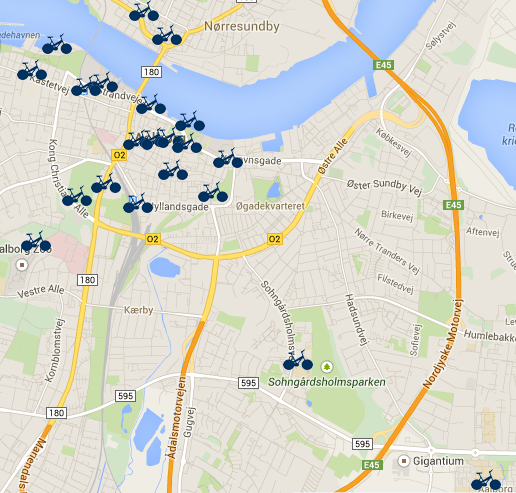
\includegraphics[scale=0.75]{analysis/CykelLokationer}
	\caption{Bicycle locations \citep{misc:aalborgbycykel}.}
	\label{fig:CykelLokationer}
\end{figure}

In 2009, 135 bicycles was placed in Aalborg, and in 2012 this number had been increased to 200 bicycles \citep{misc:aalborgcykling}.
In order to borrow a bicycle, you need to go to one of the bicycle stations, deposit 20 DKK to unlock the bicycle, then return it to a station when you are done with the bicycle, where you then retrieve your 20 DKK, which makes the system free to use \citep{misc:aalborgbycykelregler}.
The system is built on trust, because if people do not return the bicycles to a station when finished using them, the bicycles gradually disappear.

\bycykel has had, as of 2012, success with their system. 
According to a report, if the system had not been in place more than half of the users would have walked and 5 percent would have driven in a car instead \citep{misc:aalborgcykling}.
Furthermore, it shows that over three seasons the percentage of bicycles lost have been at maximum 11\% \citep{misc:aalborgcykling}.

As the bicycles are borrowed by depositing 20 DKK, no consequences exist for not returning the bicycle except for losing the deposit.
This can lead to bicycles getting lost and as there is no additional monitoring of where the bicycles are located around the city, other than travelling around the city to locate the bicycles, which is a problem.
Another problem of not monitoring the position of the bicycles is that it can be difficult for Aalborg Kommune and the potential users to know which stations have bicycles.

On the website of Aalborg Bycykel shows that a way for them to locate misplaced bicycles is through people reporting lost bicycles by way of SMS and voice mail, or by returning the bicycle themselves claiming the 20 DKK \citep{misc:aalborgbycykelmangler}.
However, if a lost bicycle is not reported or returned by someone, the bicycle is practically lost.
The company AFA JCDecaux is in charge of bicycle maintenance and storage during winter time and is also the company in charge of retrieving the lost bicycles \citep{misc:aalborgcykling}.

\subsection{Meeting with Aalborg Kommune}\label{subsec:meetingaalborg}
In order to gain more information about \bycykelwithoutspace, a meeting with Aalborg Kommune was conducted. 
Through this meeting various information was found that is kept in mind when developing the system.

For the overview of bicycles, it was found that Aalborg Kommune has no control over and little actual knowledge about the usage of the bicycles when they are placed at docks in Aalborg during the season.
The only information they get is if they see somebody bicycling in the city, or if a person makes a phone-call regarding a bicycle.

We asked them if they had received any complaints, if so what those complaints consist of.
This lead them to talk about how they are interested in information about the usage of the bicycles.
They said that the complaints they get is mostly about bicycles not being available.
Additionally, they said they often see empty stations themselves.
They thought that GPS tracking could be interesting, to monitor the bicycles and see how the bicycles are used, indicating that some administrator page is useful.

Additionally, we asked them if they have had any thoughts on booking of bicycles.
They told us that they had not thought of that but are open to the idea.
However, they can also see some cons for such a system, namely that it could become too restrictive for the user since bicycles have to be made unavailable from free access because of bookings.
They think of the usage of the bicycles as a spontaneous action instead of something the user plans to do.
However, the system is not strictly developed for Aalborg Kommune alone but more on the focus of the users of the system, and as such, the booking system can still be of use.
Whereas, the administrator part with statistics is aimed to be used by Aalborg Kommune.

%These problems could possibly be resolved, and to find inspiration to a solution, other existing systems are analysed.
	\section{Other Existing Systems}
A part of analysing and designing a city bicycle system is to investigate the current solutions on the market. 
Therefore an evaluation of existing systems is conducted.
We found several existing systems implementing different aspects and features of a city bicycle system. 
These systems are listed below:
\begin{itemize}
\item Bycyklen in Copenhagen (gobike)
\item Cibi by AFA JCDecaux
\item Alta Bicycle Share
\end{itemize}
\subsection{Bycyklen in Copenhagen}
The bicycle share system in Copenhagen is called Bycyklen and contains 1,860 bicycles and 100 docking stations \citep{misc:bycyklen}. 
Gobike is a Danish/Dutch company that designed this smart system with a bicycle they call Smart Bike. 
The Smart Bike is equipped with an information screen in the form of a tablet providing the user with an interface to lock the bicycle, select the level of assistance from the electrical system, navigate through the city via GPS and explore new interest points such as cafés and shops.
Furthermore, users of the bicycle system are able to check bus or train arrivals near their current location.
The Smart Bike uses the GPS to send the location, who is travelling, and other statistics about the bicycle such as battery life to Gobike Admin.
Gobike is currently looking at possibilities such as location based marketing, and adjusting the traffic lights according to the cyclist based on the pattern of the bicycle trip and also the weather such as wind speed.
Bycyklen has a very simple 3-step process to rent a bicycle.
\begin{enumerate}
\item Book a Smart Bike ahead from your computer or tablet, find a Smart Bike and log in via the on-board tablet.
\item Unlock the bicycle through the tablet, drive around in the city, possibly assisted by the GPS, paying by the hour.
\item Return the Smart Bike, lock the bicycle and log out of the system via the tablet.
\end{enumerate}
The Smart Bike enables the user to lock the bicycle and securely park it during the bicycle trip.

\subsection{Cibi By AFA JCDecaux}
The Cibi city bicycle system relies on SMS, where a booking of a bicycle is performed by sending a SMS to a special number with the ID of the bicycle slot in the docking station \citep{misc:cibi}. 
The user then receives an acceptance SMS and the bicycle is unlocked or released from the docking station. 
A bicycle trip is charged by the hour, and as with the bicycle share system in Copenhagen, a user can lock the bicycle during the trip. 
This is done through a wire lock which uses a code that the user was given in the SMS when booking the bicycle.
The system also allows for checking the amount of bicycles at a station using special docks and chips on the bicycle \citep{misc:omcibi}.

\subsection{Alta Bicycle Share}
Alta Bicycle Share is a company that design, deploys and manages bicycles in USA \citep{misc:AltaBicycleShare}.
The company currently have projects ongoing in nine different cities in USA, with more than thousands of stations and over tens of thousands bicycles. 
Alta Bicycle Share believes that humans get the best experience from the environment when the environment is sustainable and enjoyable.
The bicycle stations are designed such that they can be placed everywhere in the cities without doing any preparation, since they get electricity from solar panels.
Furthermore, the stations are using a cellular connection to upload their data to the main database, so the citizens can see if there are any bicycles at a given station.
To rent a bicycle from one of Alta Bicycle Share's system, you have to use a card, which can be brought in shops near the stations.
These cards then give access to any bicycle for a given time at any station, however, using the bicycle for a longer period of time can lead to a fee.

\subsection{Summary}
The Copenhagen city bicycle system, GoBike, have some good features such as a booking system that works using a tablet on the bicycle that is connected to the internet.
It also includes a GPS used for navigation and tracking.
A downside to this is that tablets cost a lot of money and need to be secured such that they can not be stolen. 

Cibi is a little different in that booking happens over SMS.
At the same time it also allows for locking of the bicycle using a special code also sent over SMS.
It also allows for retrieving information about the amount of bicycles at a station using a special dock and a chip on the bicycles.

Alta on the other hand uses a card to rent bicycles and it uploads information about bicycles at stations for the users of the system to more easily get an overview of where bicycles are located.

\begin{table}[h]
	\begin{tabular}{|p{0.13\textwidth}|p{0.18\textwidth}|p{0.18\textwidth}|p{0.18\textwidth}|p{0.18\textwidth}|}
		\hline  & Aalborg Bycyklen & Copenhagen GoBike & Cibi & Alta Bicycle Share \\ 
		\hline Booking & No & On a tablet & No & No \\ 
		\hline Borrowing/ unlocking & Deposit 20DKK & Login with tablet &  SMS code deposit 300DKR & Keycard \\ 
		\hline Tracking & No & GPS & Dock + chip at stations & No \\ 
		\hline Penalty & You do not get the 20DKK back & Continues payment & You do not get any of the 300DKR back & Fine per half hour overtime \\ 
		\hline Cost & Deposit, but otherwise free & Pay per minute & First hour free, then pay per minute & Depends on membership \\ 
		\hline 
	\end{tabular} 
	\caption{Comparison of bicycle systems.}
	\label{tab:bicyclecompare}
\end{table}

A comparison of the different bicycle sharing systems examined can be seen in \tabref{tab:bicyclecompare}
As can be seen, \bycykel is lacking a lot of features compared to the other systems and signifies a room for improvement.
The improvements to be performed is then inspired by the other examined systems.
However, \bycykel is free to use as long as you deliver back a bicycle after use. 
This ease of accessibility of \bycykel we find valuable, and is a value we seek to keep in the developed solution.
This insight is kept in mind for defining the problem definition and the specification of the requirements for the new system.
	\section{Problem Definition}
With the analysis of \bycykel and other similar existing systems performed, it indicates that there is room for improvement.
This leads to the declaration of the problem definition.
It is found that \bycykel is very basic when it comes to technologies, and does not utilise the internet.

In the similar existing systems, GPS, SMS, and card registration is used to locate bicycles.
Furthermore, booking is possible in several of these systems.
This gives inspiration to improvements that can be performed regarding \bycykel, and leads to our hypothesis which is defined as follows.

\begin{center}
\textbf{It is possible to develop a system that makes it easier to use \bycykel, within the context of Internet of Things.}
\end{center}

In order to verify this hypothesis, the following questions have to be answered:

\begin{enumerate}
	\item What are the requirements for a city bicycle booking and positioning system?
	\item How can the booking and positioning system be designed and implemented?
	\item Why should the developed system be used over the currently used system?
\end{enumerate}
	\section{Requirements}
A few criteria have been made, that a system for the Aalborg city bikes should be able to fulfil. In addition to this, the requirements were put into two categories, simple and advanced, and developers should prioritise simple requirements before advanced ones.

Simple:
\begin{itemize}
\item Be able to see how many bikes are available at a given station.
\item Be able to generate data for statistical analysis.
\item Give the possibility of booking a bike, so the user is certain that one is ready at the chosen station.
\end{itemize}

Advanced:
\begin{itemize}
\item Track bikes through fx GPS
\item Predict availability of bikes depending on placement and other variables
\item Use predicted availability to improve booking system.
\end{itemize}
	\section{Target Audience}\label{sec:ta}
The target audience for this project are the regular users of \bycykelwithoutspace, such as tourists and other people in Aalborg that do not have other means of transportation immediately available to them. 
Thus, we strive to develop a system that meets their needs.
In that category goes low-cost and easy access for tourists.
In general we strive to develop the booking part of the system for users who are not particularly tech-savvy, because if the solution works for them, it probably will for most other users as well.

Additionally, the organizations running \bycykel are also part of the target audience, and is kept in mind for the administration part of the system.
	
	\chapter{Suggested Solutions}
	Various suggested extensions for the current system are proposed.
	These solutions are then in turn examined and evaluated, in order to determine if a solution is preferred to others and gives valuable information for the software system.
	An exception to this is the Booking Software examination, which makes a concrete choice on what solution choose.
	\section{Availability of Bicycles}\label{sec:availability}
One of the requirements was that the users of the system need to be able to \textit{see how many bicycles are available at a given station}.
This section covers the suggested solutions for that requirement.
We will look at four different availability checking solutions:

\begin{itemize}
\item Camera based
\item Dock based
\item Chip based
\item WiFi based
\end{itemize} 

Finally we will choose a solution to implement.

% Camera
\subsection{Camera}
A solution with little technological implementation required, would be to use a camera such that users of the system can visually check if any bicycles are available at a given station. 

This solution is good because it is an easy way to add some kind of availability checking without investing in a larger system.

Of course this solution has its downsides, because the information is not reliable in certain situations. 
One example of a situation where a camera would be insufficient would be if it was dark at the station.
You also have to consider that the information transmitted by the camera can be deceiving in that it could show a bicycle that does not really belong at the station and that would make the user come to the conclusion that there are bicycles at the station.
In summary the data is not concise in that it does not provide a standardised way of looking up the information, but rather leaves it up to interpretation for the user.

% Dock
\subsection{Dock}
Another solution that requires a bit more technological implementation is a Dock based implementation.
The main idea is that when a bicycle is delivered at a station it is placed at a dock.
Where a given dock, with some solution that could be a scale or lock-detector, is then able to register if there is a bicycle located at it.
Each station then contains several docks, and can read from each of them to provide a number for how many bicycles are located at that station. 

%good:
% exact information about how many bikes are available
This solution, unlike the camera solution, provides exact information about how many bicycles are available at a given station with nothing up to interpretation for the user.

%bad:
For this system to work, the bicycles would have to be placed into the docks to provide any correct information.
That is, the system not registering bicycles misplaced outside the docks.

% Chip
\subsection{Chip}
A similar solution would be to use chips, such as RFID chips. 
Such a solution is similar in that it provides the same information, the amount of bicycles at a given station.
The solution differs, however, in the way this is registered.

One way to do this would be to take inspiration from a car park.
The station would have one or more entrance gateways and one or more exit gateways.
When entering the station with a bicycle, the total amount of bicycles will then get incremented, and when leaving with a bicycle it gets decremented.

Another way depending on the distance these chips could be read from, it would be possible to just deposit the bicycles at the station and the station would continually count the amount of bicycles it detects in the near-distance.

% good
These two solutions have in common that they are easy to use, as you come and pick a bicycle and then return it when you are finished.
% bad
On the downside it requires modifying all the bicycles in the fleet, furthermore, if using the car park idea, the stations can end up taking more space than the other solutions. 

% WiFi
\subsection{WiFi}
Using WiFi to transmit from the bicycles to the station if it is near, is another solution that could be used.
This solution captures the bicycles located in a perimeter around the station that are on the WiFi network.

This solution provides an estimate of the amount of bicycles available at a given station.
It requires very little in terms of extra infrastructure having to be built.

However, the solution is not as accurate as previously mentioned ones, as bicycles that are already being used but is near the station are registered as well.
Furthermore, it is unclear what costs would be involved with this system and how the bicycles would be powered to maintain the WiFi signal for a longer period of time. 
Maintaining the WiFi signal for a longer period of time when not bicycling may not be necessary as you could assume that when a bicycle is not active, it stays at the same place.
If that is the case, it could be enough to transmit your position when near a station and bicycling, thus powering the WiFi with kinetic energy.

\subsection{Chosen Solution}


	\section{Unlock}\label{sec:Lock}
There should be a way for the user to unlock a booked bicycle when reaching the station.
This can be solved in several ways, some of these are described hereafter.
We will look at the following solutions:

\begin{itemize}
	\item Unlock on Time
	\item SMS
	\item Password Based
	\item QR Code
	\item GPS
\end{itemize}

\subsection{Unlock on Time}
This option is independent on whether or not the user is at the station at a specific time.
When the specified time frame begins the booked bicycle becomes unlocked and is then available for anyone to use.
This leads to problems in that a user arriving too early at the station will have to wait for the bicycle to unlock, and if the user arrives too late the bicycle might have been taken by another person.
However, this solution is cheap since it only needs the lock on the bicycle, and the communication with the global system, which the other suggestions need as well.

\subsection{SMS}
Whenever the user is ready to retrieve his booked bicycle, he sends an SMS to the system, and the system unlocks his bicycle.
Compared to the previous suggestion, this suggestion does not make the bicycle available to everyone, therefore if the user is too late, he can be sure that the bicycle is still available at the station.
Furthermore, if the user comes too early to the station, he is still able to unlock the bicycle and does not have to wait for the bicycle to get unlocked.
Moreover this solution is also cheap since it only needs to have a lock, some kind of receiver for the incoming SMS, and be able to communicate with the global system.
However, this suggestion is not a free solution to the user since they have to pay for the SMS, which can become expensive if the user does not have a Danish mobile subscription.

\subsection{Password Based}
When the user arrives at the station he has to enter a password at the station to unlock a bicycle.
To be able to do this it will require additional hardware at the station to make it possible to input a password to the system.
Therefore this solution will increase the price of each station, as the additional hardware has to be located at every station.
However, it solves the issue that it can become expensive for the user, as this suggestion only costs something for the organizations behind Aalborg Bycykel.

\subsection{QR Code}
In order to unlock a booked bicycle the user has to scan a QR code located next to one of the locked bicycles at the station.
This suggestion compared to the previous suggestions does not require any additional hardware and can therefore become cheaper for Aalborg Bycykel.
However, it does require that the user has a mobile device that is able to scan a QR code and send the information over the internet to the system. This could, however, be as expensive for a foreign user as the \textit{SMS} solution due to roaming prices.

\subsection{GPS}
This suggestion uses the GPS of a device to see if the user is close to the station.
If the user is close to the station the booked bicycle will get unlocked.
To use this suggestion the user is required to have a mobile device which is able to send GPS information to the system.
This would require that the user has an internet connection as well.
Additionally this is very resource demanding for the users mobile device as the use of GPS prevent sleep mode of the mobile device \citep{misc:gpsbatteryusage}, which results in significantly lower battery duration.
Moreover, if the user passes by the station before he actually wants to use the bicycle there is a risk that the station will detect this, therefore unlocking the bicycle.

\subsection{Information Gain}
The different solutions provide sufficient information to the system, to be able to register when a bicycle needs to be unlocked.
Common to all but one solution is that it can be mapped to a password sent to the system, in order to unlock a bicycle.
The exception being the \textit{Unlock on Time} solution, where instead once the time runs out the lock unlocks.

\subsection{Preferred Solution}
The chosen solution should be simple for the user, without requiring specific tools, while still being usable, as specified in \secref{sec:systemCriteria}.

The \textit{Unlock on Time} solution is simple as it does not require anything from the user in terms of equipment, it does, however, have the drawback that the user has to be at the station in time of the unlocking of the bicycle.
It does not leave much flexibility for the user to arrive a little early or a few minutes late.

The \textit{SMS} solution requires that the user has a phone capable of sending an SMS. 
According to Danmarks Statistik 89\% of people aged 16-74 are able to send and receive an SMS in the year 2013 \citep{misc:dstMobilephone}.
It is expected that nearly everyone has a phone capable of sending SMS, but for tourists it might be a problem since not everyone is able to send an SMS to a foreign number or that it might be expensive.
Since the bicycles are also minded towards tourists, this could prove to be a problem.

To be able to use the QR code solution, the user would need some kind of scanner with internet connection, for example a smartphone.
60\% of the people aged 16-74 in the year 2013 was using internet on their phone, according to Danmarks Statistik \citep{misc:dstMobilephone}.
For the GPS solution, with a smartphone kept in mind, it is important that the smartphone with GPS also has an internet connection to communicate its position to the system, such that the system can react on this.
Because of the relatively low adoption of smartphones, QR code and GPS may not be proper solutions.
We are aware that other mobile devices can also read QR codes, but the device requires internet access to notify the system about the content read.

The \textit{Password Based} solution, however, appears to require more hardware installations at the stations, though it does solve the problems of the other solutions in that everyone can use it and the user is in control of when they get the bicycle.
	\section{Booking Software}
In order to book a bicycle the user need to interact with some interface.
This interface could be in the form of a website or an application, each with their pros and cons.

\subsection{Website}
The user could make their booking through a website where the user could be asked to create a profile.
The advantage of requiring a user to make a booking could be that the user, as well as Aalborg Kommune, would be able to see statistics about their bicycle usages.
It does, however, have the disadvantage that it is slightly complicated to make the booing, since the user is required to login, although with modern browsers that is able to store usernames and passwords it can make it less complicated.
If the user is not required to create a profile, then in combination with the ideas about unlocking the bicycles, discussed in \secref{sec:remoteLock}, the user would still need to enter some information that can be used to identify him and his booking.
It could be argued that in the long term it would be simpler to create a profile and login, rather than entering the same information for each booking.

\subsection{Application}
The application could be in the form of a mobile application. 
This would simplify the booking process for the users on the move, because the application could be optimised for easy access using touch screen gestures.
The mobile application would exclude people without a smartphone unless both a mobile application and a website are developed.
However, the mobile application could be in the form of a website optimised for phones, and thus allow people to easily use their phone, as well as their desktop computer for booking. 

\subsection{Chosen Solution}
For this project it was decided to focus on only one application.
We decided to focus on a website, since it can be optimised for use on mobiles phones as wells as for desktop computers. 
If the solution had been a dedicated mobile application it would limit the possible users to be people with smartphones, and possibly primarily Danish users because of the roaming prices.
We chose that the better solution was for the user to create a profile in order to book bicycles. 
This would allow Aalborg Kommune to keep better track of who was using the bicycles and the user would not need to enter their user information each time they want to make a booking.
	\section{Tracking of Bicycles}
In order to counter the loss of bicycles, tracking of the bicycles could be used.
With tracking, lost bicycles can be located and reused in the system.
Furthermore, tracking can be used for analysis of the bicycling patterns, to see where most bicycles travel to, indicating new hotspots for potential placement of new stations.
Additionally, tracking can be used to give an estimate of when a bicycle may arrive at a given station, opening up the possibility of providing waiting users with information about when a new bicycle might be ready for use.

The tracking system analysed is GPS.

\subsection{GPS}
GPS satellites are in orbit around the Earth.
GPS is for example used for navigation purposes because it provides a reasonably accurate position of objects.
For our purposes, however, it could be used to determine the position of a bicycle, though it would require some kind of GPS device being attached to the bicycle.
This could then be used to find lost bicycles.
GPS usually only works when outside, but as you are outside when you bicycle this is not a problem\citep{misc:howgpsworks}.

For each bicycle it is sufficient to have a GPS device used to determine the position and a power source for it.
Then to report the position, some connection to the developed system would have to exist.

\begin{comment}
\subsection{WiFi}
Tracking with WiFi is another technique that could be used \citep{article:wifitracking}.
The idea here is to place beacons around the city.
The beacons can then retrieve WiFi signals from a bicycle, and use this to determine the location of the bicycle by making the beacons report when bicycles connect to then.

An advantage of this type of tracking is that you are not dependent on some external beacons you do not own.
The downside of this is that you would have to place beacons all around the city of Aalborg in order to precisely locate a bicycle.
Furthermore, you would need a WiFi module on each bicycle, and as such you increase the amount of equipment needed to track the bicycles.

\subsection{Information Gain}
Both solutions provide the same information, which is the position of a bicycle at a given time.
As such, from a software point of view, both solutions are sufficient.
However, from a hardware point of view, the GPS solution is preferred, as it requires less equipment than the WiFi solution. 
Moreover, the GPS solution still needs some means of connection to a server in order to send the location of the bicycle \citep{misc:gpsSystem}. 
This connection could be established, for example through a cellular network which is inspired from Alta Bicycle Share, see \subsecref{subsec:alta}.
\end{comment}
	\section{Chosen Solution}
To provide the project with valuable information about how the system could work in the real world, we also choose a solution for the hardware elements.
This is despite the fact that only the chosen software solution is implemented, which is the website, the interfaces and the simulated hardware elements.

For the availability of bicycles, we choose to use docks since it also covers part of the hardware aspect of a different requirement, being able to lock.  
For locking we also choose to use passwords that need to be input at the station because it is something everyone can do once the booking has been done, as SMS, QR codes, and GPS require phones and might not be suitable for tourists.
For tracking of bicycles we use GPS.

The following provides an overview of the chosen solution using rich pictures.

The server-station relationship is shown in \figref{fig:ServerRichPicture}.
It depicts a central server, where the different bicycle stations are connected to.
Furthermore, people can access the website to gain information e.g. bicycle count, but also to register bookings, where the server then communicates this to the given station(s).
Those stations then takes care of locking and unlocking bicycles to satisfy the bookings performed.
The server contains all information about each station, such as bookings, amount of available bicycles at stations, and usage statistics.
It provides booking and amount of available bicycles at stations through a website to the user. 
Usage statistics are provided to the facilitators of the system and gives them the ability to improve the system. 

\begin{figure}[h]
\centering
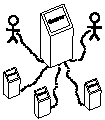
\includegraphics[scale=3]{serverrichpicture/server.pdf}
\caption{The server and the associated stations.}
\label{fig:ServerRichPicture}
\end{figure}

The dock that provide the locking and unlocking mechanism along with the bicycle detection ability have to communicate with the station. 
This is for example when they need to unlock a booked bicycle, the information needs to be propagated from the station to the individual dock containing the bicycle.
A sketch of how a station could look like when deployed can be seen in \figref{fig:StationRichPicture}.
The figure depicts a station and two docks connected to the station, which contains a bicycle each. 
On the display of the station, it can be seen that two bicycles are available for use.
\begin{figure}[h]
\centering
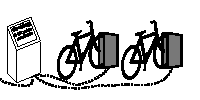
\includegraphics[scale=3]{stationrichpicture/station.pdf}
\caption{The station and the bicycles.}
\label{fig:StationRichPicture}
\end{figure}
	
	\chapter{Technologies}
	Some background material is needed for the development of a solution and this is examined and discussed. This includes describing the Internet of Things and what issues follow that, a description of the Model-View-Controller pattern used for the website, and AJAX(aka dynamic updating of websites). \fxwarning{Skal ER-Diagram være her?}
	\section{The Internet of Things}
This section introduces the Internet of Things (IoT), along with examples of how it is used. The section also introduces various hardware considerations to provide the context in which real-world applications for the IoT are developed.

The IoT is the concept describing the interconnection of uniquely identifiable objects in the problem domain.
The IoT also includes the virtual representation and the interfaces that allow for manipulation and information retrieval regarding objects \citep{misc:InternetOfThingsDefinition, misc:InternetOfThingsDefinition2, misc:InternetOfThingsDefinition3}.

Real usage of the IoT manifests as systems to provide some service, either by informing the user regarding things or allowing an intelligent system to manage those objects.
An example of this could be a so-called `smart home' that allows you to use a single device to manage the connected objects in your home, such as the lights or the oven in the kitchen \citep{misc:InternetOfThingsExamples}.
One society-wide use for it is the idea of a `Smart Grid', where the electricity usage is monitored and managed by an intelligent system that will e.g. redirect electricity if a cable has been cut somewhere in the system \citep{misc:smartGrid}.

There are already a lot of objects in the IoT, and by 2020 it is estimated that there will be upwards of around 26-30 billion things \citep{misc:IoTGrowth1,misc:IoTGrowth2}.
This will likely require a jump to the IPv6 protocol as the amount of IP addresses are severely limited by IPv4 \citep{misc:numberOfAddresses} given that the additions to IPv4, such as multiple devices sharing a single IP address, will at some point become insufficient.

One important aspect of the things connected to the IoT will be what technology they use to connect, here WiFi or mobile networking will not work well as they will likely interfere with one another.
The connectivity technology has to be low-power, cheap, and non-interfering.
One way to do that would be to directly connect objects to a server with a cable connecting to the internet, though that is not practical for objects that must be mobile.
RFID (Radio Frequency Identification) chips can provide relevant information to an outside observer about the object itself \citep{misc:rfid} with active research in making it low-cost and low-power \citep{misc:rfid2}.

The geographical location in the IoT is a good idea, especially for sensors where the location provides important context for the information of which something is accessing \citep{misc:locationMatters}.
For example if there is a station for bicycles in a bicycle sharing system that needs to provide information regarding the amount of bicycles at the station, it is important for the usage of the information that it also provides the actual location of the station, if that is not otherwise known.

In order to give more detail on IoT, aspecs about identification, communication, and software is given.

\subsection{Identification}

\subsection{Communication}

\subsection{Software}



In summary, the IoT has many challenges but at the same time also provides opportunities and benefits for society in general.
There are of course also criticism to it, primarily from a privacy point-of-view because it provides too much information.
	\section{Model View Controller}\label{sec:mvc}
The Model View Controller (MVC) is a design pattern widely used in programming to separate the program into Model, View, and Controller.
This provides the advantage that the code gains clarity and is easier to maintain as it separates responsibility to individual layers.

An illustration of MVC can be seen in \figref{fig:MVC}.
\begin{figure}[h]
	\centering
	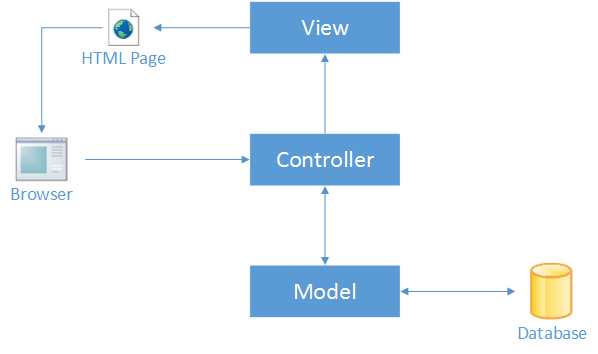
\includegraphics[scale=0.6]{relevantmaterial/MVC}
	\caption{Illustration of MVC pattern.}\label{fig:MVC}
\end{figure}

If you look at the illustration, the `Database' is in our case the relational MySQL database, where data is stored in tables.

The `Model' in our case provides abstraction over the information in the database, it consists of several entities and a service for each such entity.
This is to make the entities simply wrap data, while the services work on the data, and each implement an interface, requiring the services to implement Create, Read, Update, and Delete (CRUD) methods.

The `Controller' provides a set of 'actions' that the user points the browser at. 
These actions then use CRUD methods in the `Model' layer and can also send commands to views to update the view's representation of the model, e.g. a table or a map of stations. 
These views are then presented to the user through the client.
A controller may include multiple views to get a html-page generated for the client to view.
As multiple views may be included by the controller, it may use separate views for the header, the body, and finally one for the footer.

It is important to note that there is a single model layer, consisting of multiple entities (e.g bicycle and booking) and their associated services.
Additionally, it is a good practice to have multiple controllers, which each handle different parts of the website.
In our case we for example have a home and user controller.
With the user controller taking care of everything connected to user login, editing of profile, logout etc.
The home controller takes care of the presentation of the frontpage and the functionality of booking and unbooking of bicycles.
As is evident, the controllers are split into different actions present on the website, which ensures better code clarity.

In addition to the better code clarity, as the website is organised in the way it is, working with the same model, the layout of the website can easily be changed, by including other views or developing additional controllers for other work routines.
This is relates to the high modularity you gain with the MVC pattern, inducing high cohesion and low coupling.
	\section{Asynchronous JavaScript and XML}
Asynchronous JavaScript and XML (AJAX) is a way to create a website update parts of the website without user interaction.
By using AJAX, parts of the websites can be updated without reloading the whole website every time, which makes the user experience of a website much more smooth.
Even though XML is a part of the AJAX name, it is not necessary to use when using AJAX, other methods to send the data can be used, an example could be to use JSON.
When using JSON, data is encoded and then displayed on a page by itself, which the javascript then decodes and can use to reload the affected parts.

The reason to use AJAX is to improve the usability of a website, as well as the performance of a page.
An example of this is e.g. when rating a film on www.IMDB.com then when pressing the rate, the website does not reload, but instead calls for an asynchronous update to the database giving the user an non-interrupted experience. \fxnote{kilde her}
AJAX should be used whenever the user interacts with something that does not need to update the entire page, but only update information on the database, this could be changing the password of a user or it should be used when updating only a part of the website, so that the website should not be refreshed before updating this part of the website.
    \section{Simple Object Access Protocol (SOAP)}
The \textbf{S}imple \textbf{O}bject \textbf{A}ccess \textbf{P}rotocol (SOAP) is a protocol for sending structured messages over a computer network using XML.\citep{misc:soapintro}
The use of a SOAP helps structuring message passing, providing type information for contents. 

SOAP is useful because at the same time as allowing transmission of information, it also allows implementation of functionality for what is to be done once that information has been received.

A reason to use SOAP over other methods for transmitting information is because it provides more possibilities for security and is generally considered more reliable, and because it provides a standard use that makes it easier for new developers to pick it up. 
SOAP is generally considered slower and much more verbose than other methods.
Other methods on the other hand are generally more versatile when it comes to complex types, and is generally simpler, much less verbose and faster.

We chose to use SOAP because while other methods are less verbose, faster, and simpler, SOAP provides a standard protocol that while complex and verbose is a very big benefit.\citep{misc:understandingsoapandrest, misc:restsoapwhen}
		
	\chapter{Design}
	This chapter will present the design of the product, where a prototype is created hereafter the ER-diagram of the database is explained.
	%!TEX root = ../../main.tex
\section{Website Prototype}\label{sec:prototype}
In order to get a better idea of how the website should look like, various prototypes were drawn.
As they are prototypes, they are by no means a representation of the final product, but more of a source of inspiration and brainstorming, to consider when developing the website.
Throughout this section, prototype sketches for different parts of the website, is presented, explained, and discussed.
Our primary inspiration is based on the current website for \bycykel \citep{misc:aalborgbycykelMain}.

For all the prototypes presented in this section, the arrows on the pages have been drawn with different styles to distinguish between different actions. 
If two arrows have the same style it means that they are associated with one action following the other.
Additionally, the prototypes presented are for the booking part of the website, with the administration prototypes omitted, as those were quick sketches on a blackboard.

\begin{figure}[h]
	\centering
	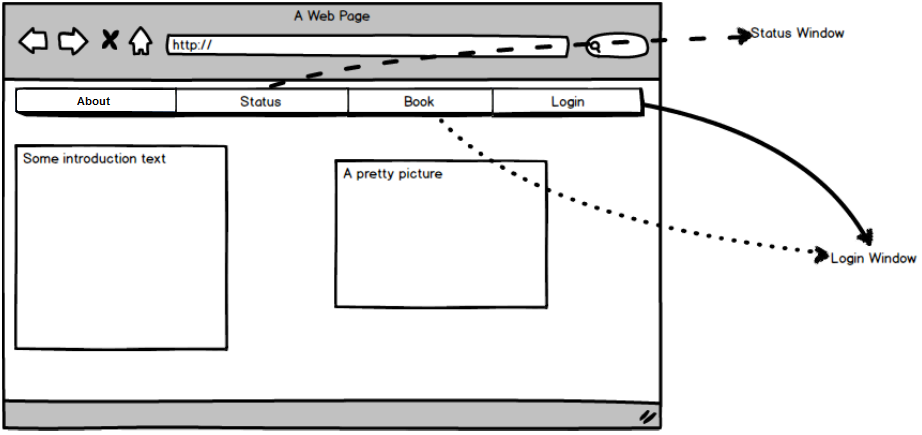
\includegraphics[scale=0.6]{design/prototype-about}
	\caption{About page.}\label{fig:prototype-about}
\end{figure}

 
First, we take a look at \figref{fig:prototype-about}.
This illustration presents a draft of the about page, it is structured as a standard about page with some description of the organisation behind the website.
What is more interesting to see in this illustration is the first draft of the menu bar.
The menu bar consists of links to about, status, book, and login, each of which have their page(s) illustrated hereafter.

\begin{figure}[h]
	\centering
	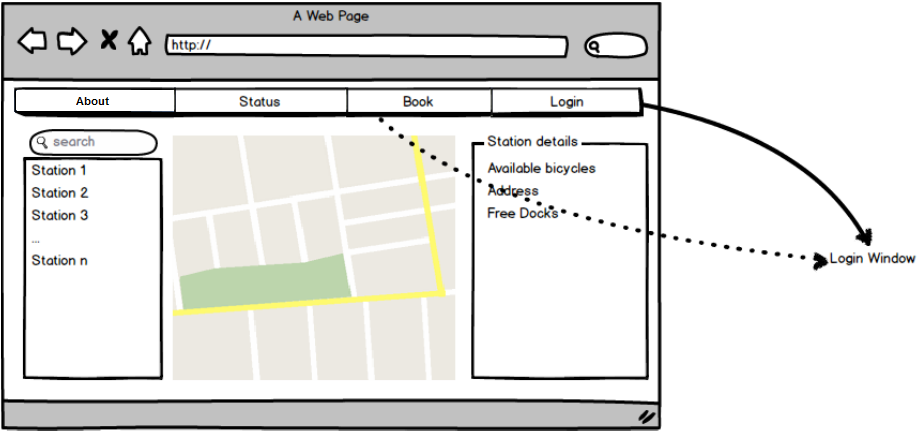
\includegraphics[scale=0.6]{design/prototype-status}
	\caption{Status page.}\label{fig:prototype-status}
\end{figure}

Next is a presentation of the status page, see \figref{fig:prototype-status}.
The main idea is that the status page should be easily accessible and is what should be shown when navigating to the homepage.
The reason for this is that the status page should easily be able to give you an overview of the status of each station.
As can be seen from the illustration, this station detail can be found by selecting a station from a table, searching for it, or selecting the station on a map.
When a station is selected, details are shown for it, which can be useful to see if available bicycles exist at the station.
In many ways, the status page is similar to the booking page, which is presented hereafter.

\begin{figure}[h]
	\centering
	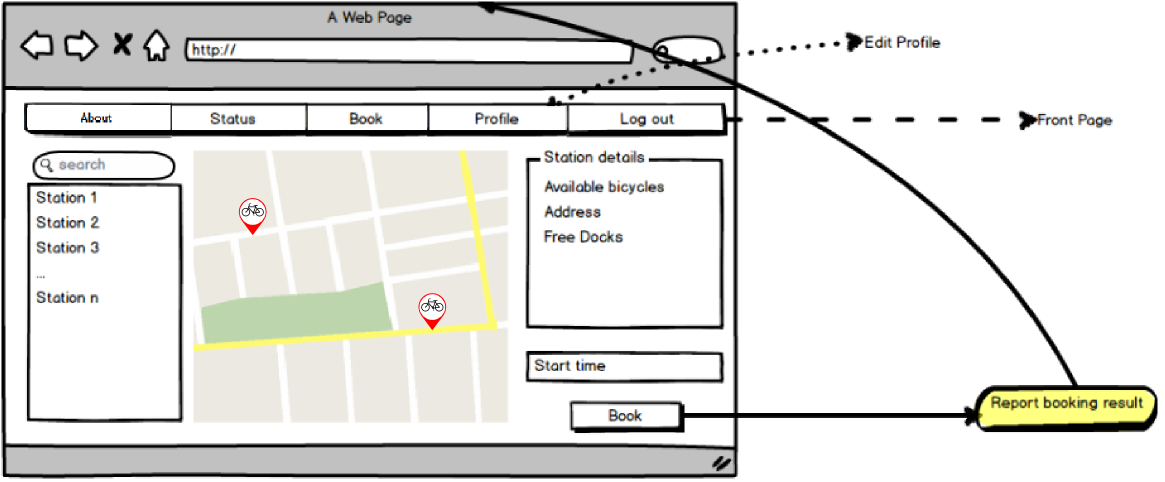
\includegraphics[scale=0.5]{design/prototype-booking}
	\caption{Booking page.}\label{fig:prototype-book}
\end{figure}

For an illustration of the booking page, see \figref{fig:prototype-book}.
The booking page can only be navigated to if you are logged in, if not you are redirected to a login page.
The booking page is otherwise the same as the status page, except you are able to book a bicycle at a given time.
To make a booking, you would login to the website and navigate to the booking page.
Thereafter you would select a station where you want to book a bicycle and select start time, which is the time you expect to retrieve the bicycle.
When you then click \textit{Book}, the booking result is handled and registered in the system if valid.

Prototype pages also exist for the profile login and management, but has been omitted as these pages are very standard pages.
In that meaning one page being a login form and another page being a form with some fields to edit your password, phone, and email.
What is interesting though, is that you can access your booking history page through the profile page.

\begin{figure}[h]
	\centering
	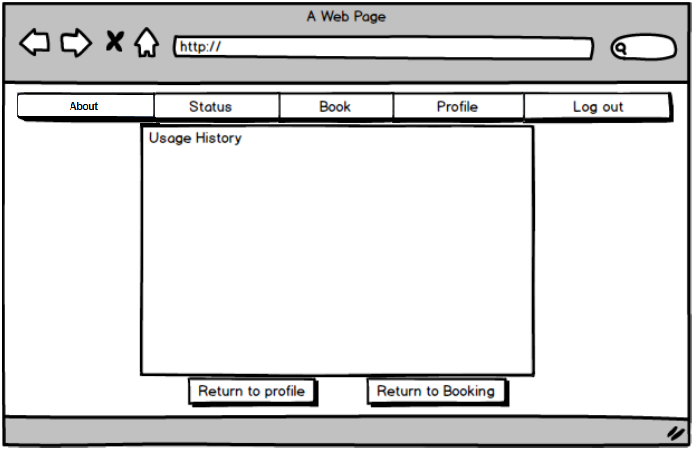
\includegraphics[scale=0.6]{design/prototype-usage-history}
	\caption{Booking history page.}\label{fig:prototype-usage-history}
\end{figure}

The booking history page can be seen in \figref{fig:prototype-usage-history} and shows your whole booking history.
The booking history is thought useful because it might be reassuring to show the user that their bookings have been handled correctly by the system and to generally support users that think that their actions have not been properly registered.
Furthermore, sometimes you see webshops provide purchase histories, and you can for this page consider a booking a metaphor for a purchase.

This ends the description of the prototypes for the system, and is what we first had in mind before implementing the system, and as of such you will later see some parts of this used for the implemented system.
	\section{Entity--Relationship Diagram}
In order to have an idea of how the database handles bookings, location of bicycles, and their relation to the location of the stations, an ER Diagram was made, see \figref{fig:er-dia}.

\begin{figure}
	\centering
	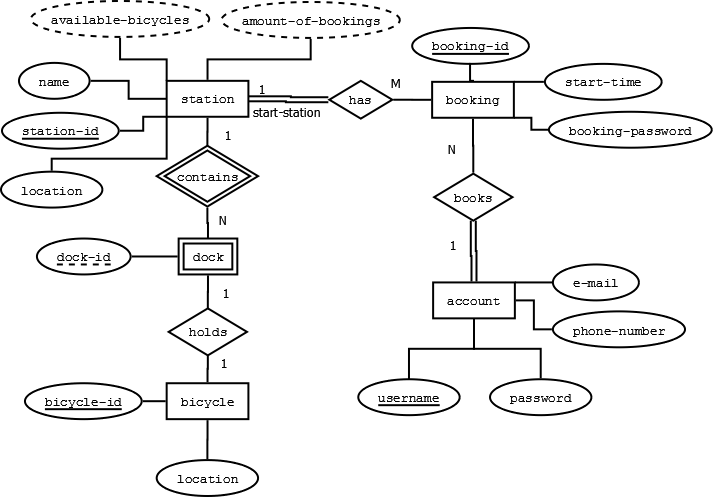
\includegraphics[scale=0.4]{relevantmaterial/erdiagram}
	\caption{The ER Diagram for database overview. Does not include less important attributes.}\label{fig:er-dia}
\end{figure}

As seen in the diagram, the entities consists of bicycle, dock, station, booking, and account.
An account consists of a username, email, which both must be unique, a phone-number, and password.
These attributes are common for an account entity, with the phone-number being special in that the idea is they will receive the booking-password over SMS.

In relation to this is the booking entity, where it can be seen that a user can have many bookings whereas a booking is registered to one and only one account.
The booking then has a booking-id, to uniquely identify a booking, a start-time, such that a station knows when to lock a bicycle, and a booking-password, used to unlock a bicycle at the given start-time if a correct password is entered.
The idea is that if a booking is not used in a given time frame at the start-time, the booking will be removed, to prevent spamming of bookings without use.

A booking is also tied to a station, such that a booking is located at one and only one station, whereas a station can have many bookings.

A station has the attribute station-id, to uniquely identify the station.
Furthermore, it has a name, which is thought to be used to give a meaningful description of a given station.
We are aware that the name could be used as a primary key, but having an id as the primary key unlocks the possibility of duplicate names, which might be desired for stations located at different spots in the city, example could be two stations named "AAU Bycykel Station" which is a quite generic name.

In addition to this, a station has a location, which is used to easily place a station on a map, and can also be used for calculations such as distance between a given station and bicycle.
A station also has two derived attributes, which are available-bicycles and amount-of-bookings, these are attributes that is beneficial to show to the user, such that they can see if it is possible to gather a bicycle at a given station.

Next is the dock entity, which is a weak entity, as it cannot exist without a station.
This represents the real-life situation with stations located around the city, and each of these has a number of docks.
The dock only has one attribute, which is the dock-id, used to identify a dock in combination with a station-id.

The interesting part of a dock is its relation with a bicycle.
A dock may or may not hold a bicycle, which is represented with the holds relation.\fxwarning{Locked docks?}

The bicycle entity then consists of a bicycle-id, to uniquely identify a given bicycle, and a location, which can be used to locate lost bicycles.
	%!TEX root = ../../main.tex
\section{Administration Tools}\label{sec:designAdminTools}
In order for the administrator of the bicycle system to make reasonable decision about future actions/improvements towards the bicycle system, statistical data has to be collected and shown to the administrator. This will give him an overview of the usage of the bicycles and prepare him to make an informed decision or just provide him with a knowledge of how the system is used.
A list of questions should be able to be answered or hinted by the system, however, the implemented features in the final system will likely be limited by available time:

\begin{description}[style=nextline]
\item[Which routes are used?] If routes could be determined, patterns could possibly be seen, e.g. if there is a particular route that is very popular.
\item[Where is the most traffic of bicycles during some period?] An administrator would be able to see how many bicycles leaves and arrives at each station and thereby get an overview of where the traffic is high and low, providing an indication of where to put focus for relocation of bicycles and expansion of stations.
\item[How does the amount of bicycles at a given station change over time?] The administrator can choose a long time interval, providing a more general overview of when the activity at each station is high or low, also providing him with an overview of usage at each station.
\item[What is the status of the stations?]
An overview page of the stations should be implemented, providing information about stations such as if they are online or not, where they are and what their status is with regards to usage.
\item[Are there hotspots for bicycles?] If positions of bicycles could be determined, it would mean that different kind of patterns could be detected, for example detecting stagnant bicycle hotspots could provide valuable knowledge about where to add new stations.
\end{description}

Keeping a log of information about the usage as described above, requires additional database tables having timestamps as an important factor since the usage of bicycles is tied to some real life events that needs to be logged. 
In order to log the routes for a bicycle, a new relation is added to the database schema storing information about longitude and latitude and of course which bicycle it is for and when it was logged.
In order to log traffic of bicycles between stations another relation is added to the schema having information about a start station and an end station for a trip along with times for each of the events (start of trip and end of trip).
Last, a relation to store the count of bicycles at each station along with a timestamp, is added to the schema.

Putting all this together, also illustrating foreign key references, can be seen in \figref{fig:er-dia-log}.

\begin{figure}
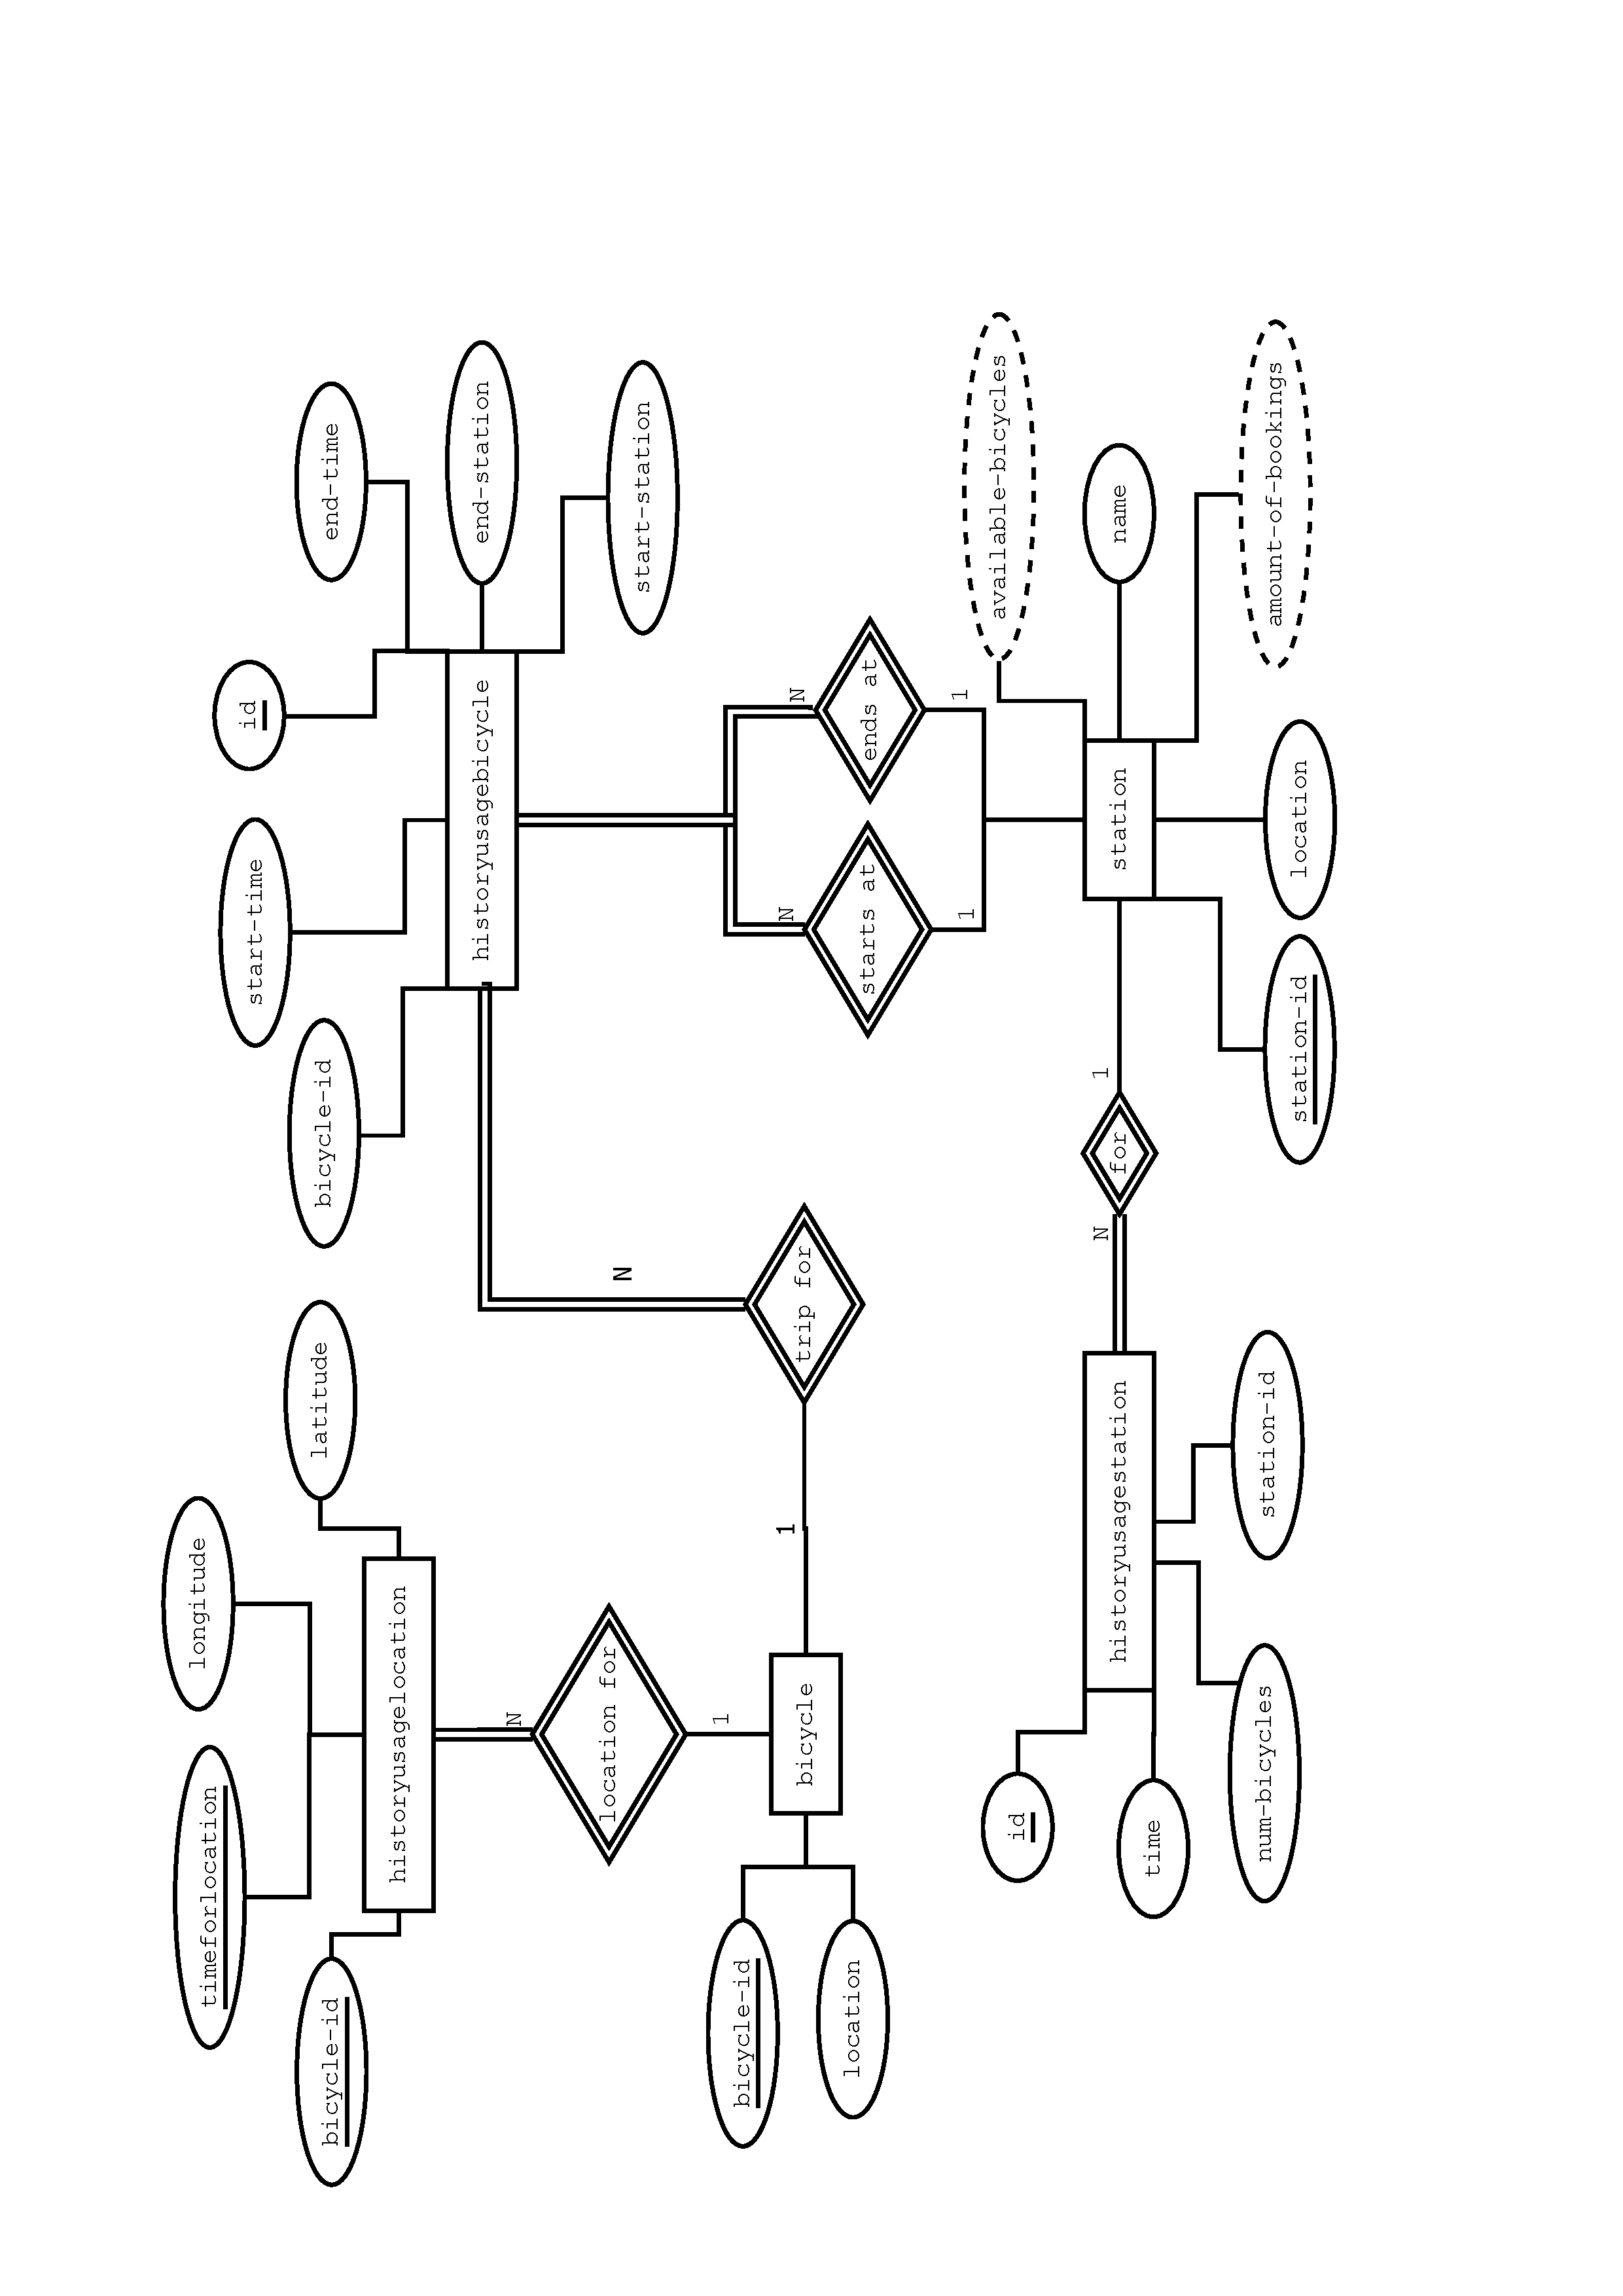
\includegraphics[scale=0.3, angle=-90]{design/ER-diagram-logging.pdf}
\vspace*{-2cm}
\caption{ER-diagram showing relations covering data logging.}\label{fig:er-dia-log}
\end{figure}

Addition and removal of bicycles, users, and stations is also part of the responsibility of the administration tools. 
For bicycles, they should be added to the system loosely and not directly to a station.
We intend to do it like this because when the administrator adds a new bicycle, they receive an id and the idea is that they use this id to program the bicycle such that it can be recognized by the system.
For users and stations, addition does not have any such considerations to make. 
The dock is not part of the administration tools, since it is handled at the stations.

Since the logging tables use the other tables like the station and bicycle tables it is important to handle deletion of stations and bicycles. 
If deletion is not handled properly the logged data could end up being inconsistent. 
In our case we handle deletion by adding a column to the affected tables indicating if the row is deleted or not, this ensures that we do not encounter foreign key constraints due to the logs referencing those rows. 
When using the station and bicycles table on the website we make sure to only use the rows that are not deleted, while for the history data we use all rows within a chosen time interval.

	\section{Architecture}
Before implementing the software system, it is a good idea to have a general overview of how the various parts of the system are connected.
In order to gain this overview, an overall architecture diagram was drawn.

The overall architecture can be seen in \figref{fig:overallarch}.
In the illustration a single arrow is a one way communication, whereas two arrows are two way communication.
The architecture is very similar to a client-server pattern, where the central database is the server, and the stations and bicycles are the clients.
As we have a central booking system, and multiple simultaneous access points, the client-server pattern is applicable and appropriate.

\begin{figure}[h]
	\centering
	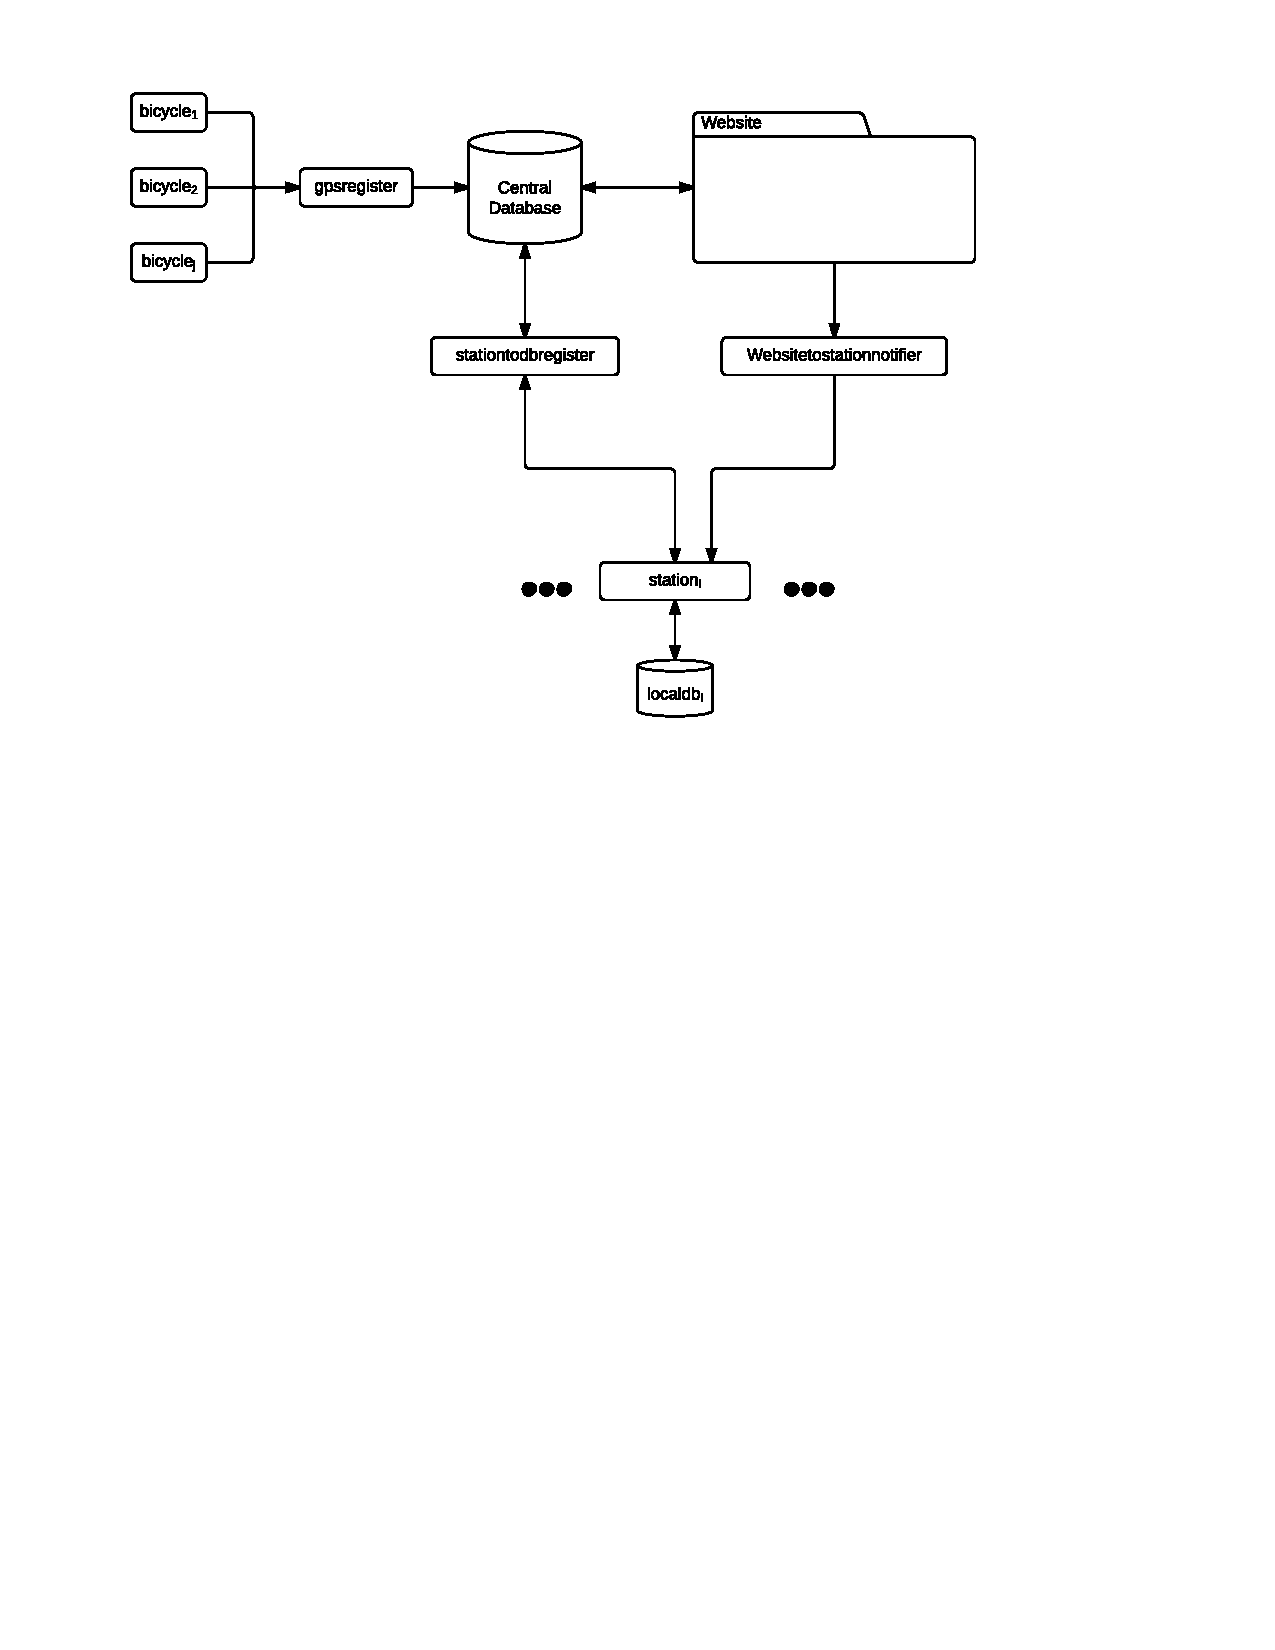
\includegraphics[trim=2cm 1.5cm 1cm 1.5cm, clip, scale=0.7]{design/architecture}
	\caption{Overall architecture}\label{fig:overallarch}
\end{figure}

As can be seen from the figure, the architecture consists of a central database as well as a website and three interfaces, named 'gpsregister´, 'stationtodbregister´, and 'websitetostationnotifier´ , where 'gpsregister´ and 'stationtodbregister´ contact the central database.
Additionally, multiple stations and their associated local database and docks exists.
The reason each station needs to have its own local database, and not merely use the central one is to minimize the necessary network communication, as well as allowing the stations to remain operational in case of network failure.
As of such, the local databases contains a subset of the central database, corresponding to the data involving the given station.
Each dock is associated with a given station, and is used by the users to take or deliver bicycles.

Additionally, the three interfaces each serves a different purpose, as described here.
The gpsregister interface, is provided for the bicycles to register their current position in the central database, as well as logging its path in another table.
This data provided can be used for route mapping and positioning of bicycles.

The stationtodbregister interface serves the purpose of updating the central database of changes performed at the local stations. Furthermore, it enables the local stations to read their subset of the central database, which is used for booting of stations from scratch, when their local database is empty.

The websitetostationnotifier is a little different, in that it is an interface provided to the website, such that when the website changes data, e.g. create a booking, the involved station is notified by the interface.

For the website part of the architecture, it is structured according to the MVC pattern, see \secref{sec:mvc}.
A detailed overview of the architecture of the controller and model part of the website are provided in \appref{app-arch:controller} and \appref{app-arch:model}

Another part of the architecture is the user interaction.
For the website, we distinguish between admin and regular users.
The admin user has access to an admin webpage, where he can modify stations, bicycles, docks, and users. 
Although a regular user can also create an account themselves.
In addition to this, the admin user is also provided with some statistics pages about the usage of the system.
The admin user also has access to the features a regular user has access to.

A regular user can interact with the system in several ways.
The website allows for station status, in order to see how many bicycles and docks are available at any given station, but also the position of each station.
In addition to this, the website also provides the option to book bicycles in advance for a given station, where the station locks a bicycle sometime in advance.
If you book a bicycle, you are provided with a password that needs to be used when you want to unlock a bicycle at the station booked at.

For the station interaction, two interactions are involved.
If you have booked a bicycle at the station in advance, you use the password provided from the website to unlock a bicycle for usage, by entering this password in the station automata.

The automata then tells you at which dock a bicycle is unlocked, and you can retrieve your bicycle.
However, if you have not booked a bicycle in advance, you do not use the station automate, but instead check each dock for available bicycles.
In that regard, we imagine a distinction between reserved unlocked bicycles and free bicycles, such that you do not on accident steal someone else's booked bicycle.

For the deliverance of bicycles, the interaction is the same whether the bicycle is booked or not.
The process is easy, as you locate a free dock and then place the bicycle at that dock.
The system will then automatically register that the bicycle has been returned to a dock at a station.

%stationer skal have egen database
%forklaring af figur
%husk teori og fancy ord, SOAP webservice er et eksempel

%uddybbelse af de enkelte komponenter.
	%!TEX root = ../../main.tex
\subsection{Station Software}\label{subsec:stationsoftdesfgi}
While \figref{fig:overallarch} of the overall architecture provides an overview of the system, the station component has its own architecture as well, which can be seen in \figref{fig:stationarch}. In this figure, as in the previous, the arrows represent flow of information.

\begin{figure}[h]
	\centering
	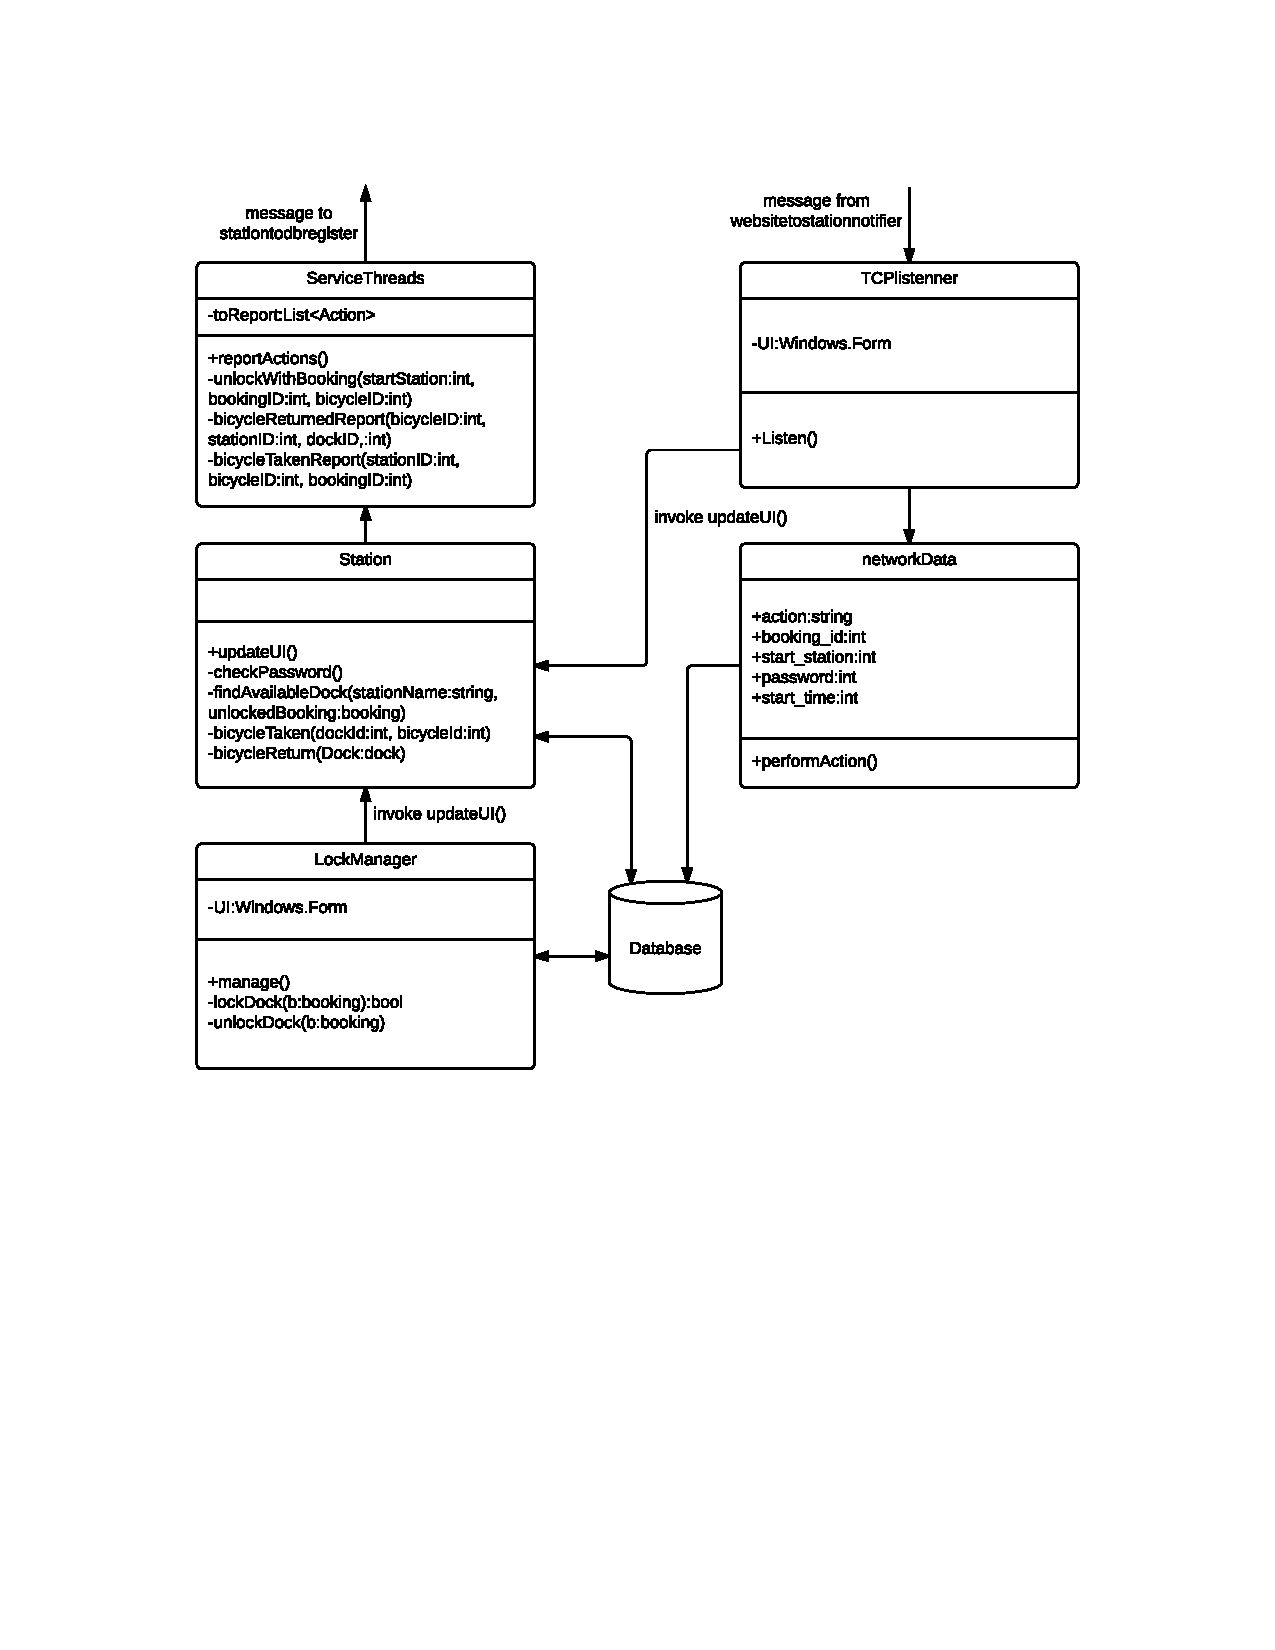
\includegraphics[trim=1cm 1.3cm 1cm 1.3cm, clip, scale=1]{design/station}
	\caption{Station software architecture.}\label{fig:stationarch}
\end{figure}

In the station software, the station is the main part and also the one that contains the UI. 
This part is responsible for all contact with the user at the station and is the one that is interacting with the hardware.

\texttt{TCPListener} is a thread that listens for messages from the global system through the \texttt{Website\-ToStationNotifier} and stores these messages as a \texttt{NetworkData} object, and tells this object to perform the action the message contains.

The \texttt{NetworkData} object has the responsibility of adding a booking to the local database corresponding to the information the object contains or removing a booking with the ID it received.

The \texttt{LockManager} is also a thread, and is responsible for locking a bicycle when a booking is close to its start time and unlocking said bicycle again if the booking's start time is exceeded by a certain limit.

The last class is the \texttt{ServiceThreads} which is also running in a separate thread.
This thread is responsible for reporting changes at the station, which are stored in the \texttt{ActionQueue} queue.
As soon as there is something in the \texttt{ActionQueue} queue, the thread tries to report it to the online interface, repeating until it succeeds in transmitting it.

However, how locking should be tackled has not been touched upon yet, but is a  central part of the system and as such is examined hereafter.

\subsubsection{Locking Considerations}\label{subsec:lockingcons}
Consider the scenario where a user $u_1$ makes a booking $b_1$ on the website at time $t_1$ wanting to reserve a bicycle for time $t_3$. Before time $t_1$ another user $u_2$ made a booking $b_2$ of a bicycle for time $t_2$. Both users made a booking at the same station, and the amount of available bicycles for that station was for both users 1. Under the assumption that a bicycle cannot be locked and thereby reserved before some amount of time, say $t_{before}$, before usage, this scenario is possible in the following way.

First consider this definition of a time $t$, it is a time represented as the number of seconds from Thursday, 1 January 1970 at 00:00:00 UTC, which is the Epoch time, as such comparisons such as $>$ is computed as usual on numbers.
Let, 
$$TSB(b) = \{(t_1,t_2) \;| \;t_1 = st(b) - t_{before} \land t_2 = st(b) \land t_1 \leq t_2 \}$$
where,
\begin{itemize}[align = left]
	\item[$st(b)$] is defined as the start time of booking $b$.
	\item[$TSB(b)$] defines the Time Span Before of booking $b$.
\end{itemize} 

\begin{figure}[h]
	\centering
	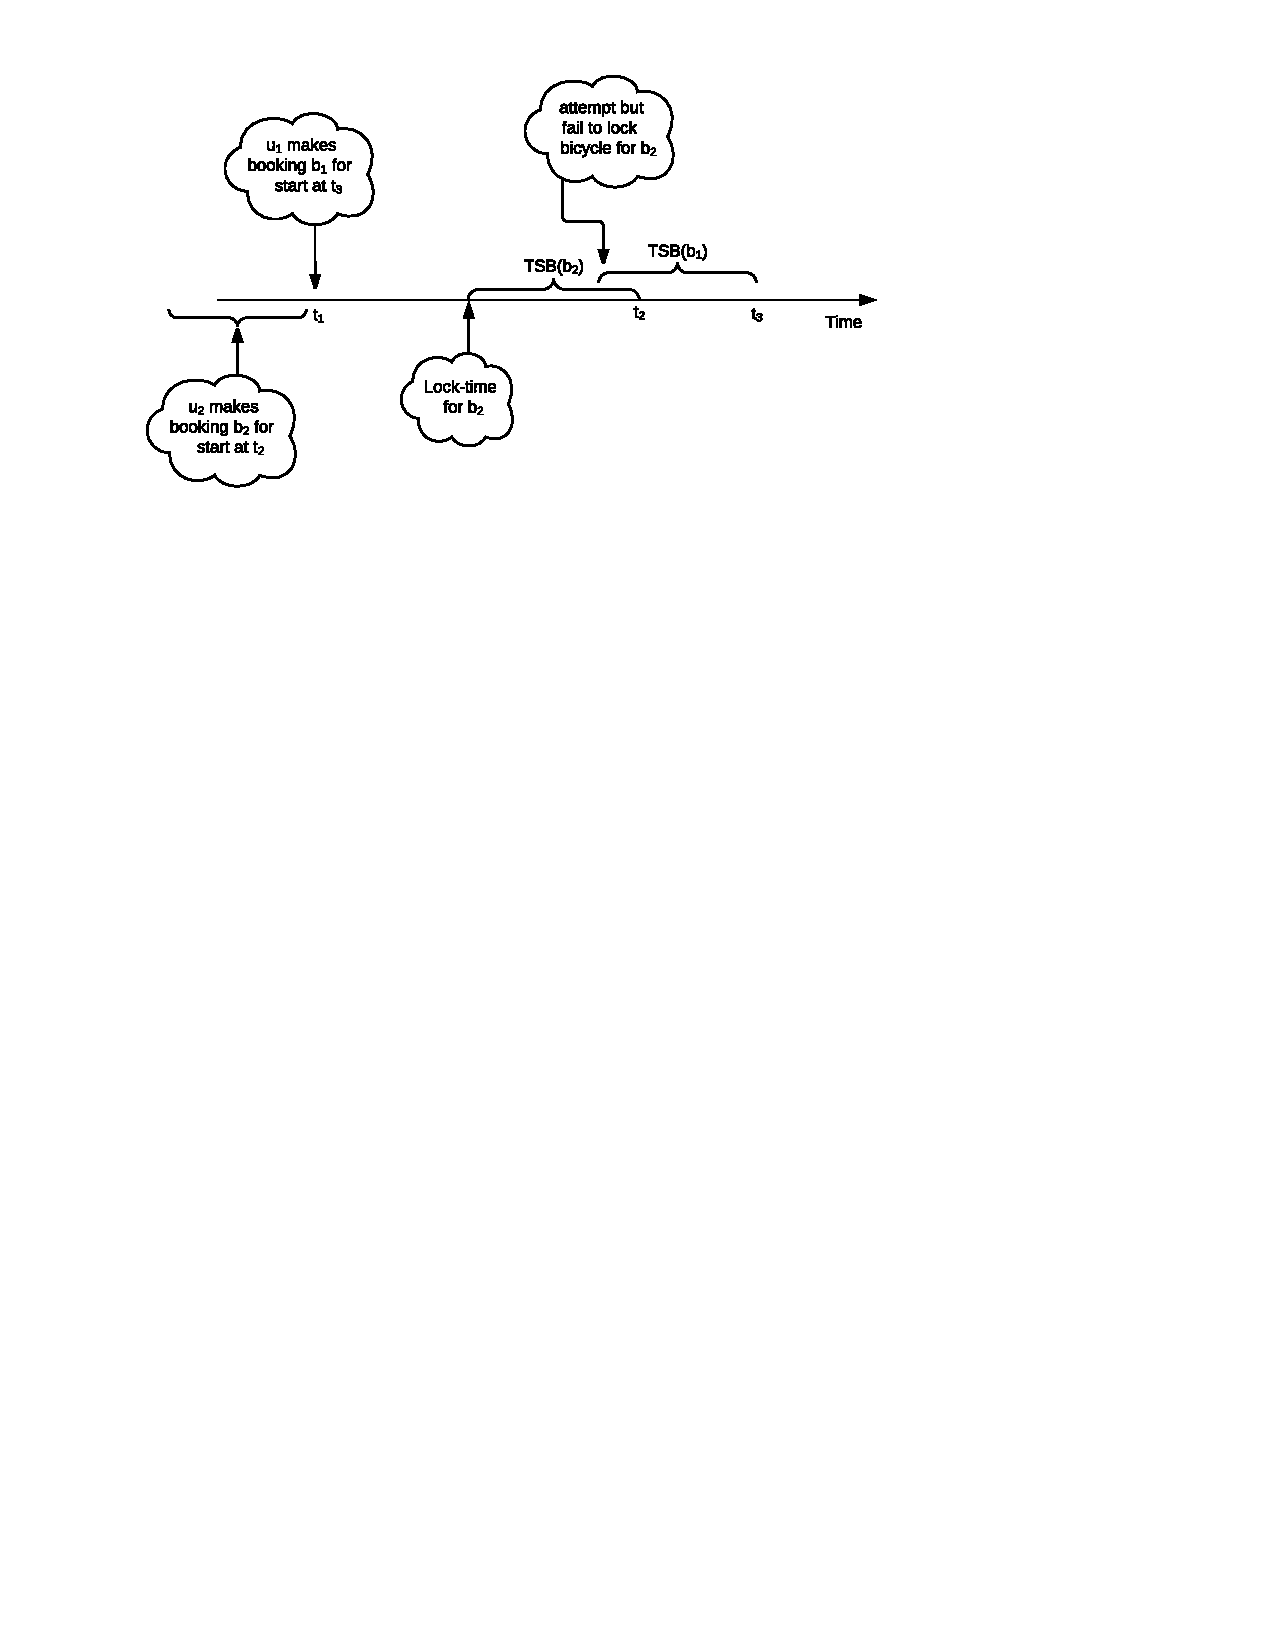
\includegraphics[trim = 1cm 19.7cm 0cm 0cm,clip]{behaviour/booking-illustration}
	\caption{Booking scenario illustration.}\label{fig:booking-illustartion}
\end{figure}
Then the scenario is given if $TSB(b_2)$ starts before $TSB(b_1)$ and $TSB(b_2)$ starts after $t_1$, we have a situation as can be seen in \figref{fig:booking-illustartion}.
As can be examined from the illustration, a problem occurs, under the assumption that no new bicycles gets delivered or taken from the given station in the given time-line, and where the amount of available bicycles before the lock-time of $b_2$ is 1.

The problem for user $u_1$ is then at time $t_1$ it appeared that a bicycle was available, but the bicycle is locked for user $u_2$ before it is locked for $u_1$ resulting in an availability count of 0 for $b_1$, thereby having no bicycle to lock for $u_1$.

The key aspect of why the handling of locking cannot be left as a responsibility of the database is to make the system less static, as requested by Aalborg Kommune, see \secref{subsec:meetingaalborg}.
If we were to make this a responsibility of the database, it would be in the case where locking should be performed immediately, but if you book a bicycle for tomorrow that would mean a bicycle would be unavailable for other users for a whole day, which is highly undesired.
An alternative would be to limit the time in advance you can make a booking, this would also increase the dynamic of the system, but would limit the booking flexibility.
This is a trade off between certainty of getting the bicycle booked and a dynamic system where more bicycles are in use.
	\section{Synchronisation}\label{sec:sync}
As the stations and the website are located on different addresses and communication is through TCP, you have to consider how to synchronise the various parts of the system, in order to avoid an inconsistent state.

Several types of such inconsistent information could happen if you are not careful.

A scenario that could lead to an inconsistent state, if not handled well, is what happens when a station fails to communicate its current state to the global system.
A station maintains a local database holding information about each current booking made at that station.
When a booking has been processed, meaning that the user has taken the bicycle associated with the booking, the state of the local database changes in that the booking does not exist any more.
This change in state is also communicated to the global database maintained by the global system.

A problem can occur when trying to communicate the change as the connection can be interrupted.
This problem is then, formulated with other words, which database will hold the correct state of the overall system?
This depends highly on the direction of communication failure. 
In the described case above, the communication failure lies with the station software resulting in the local database of the station having the correct and current state of the system, which is when it comes to the state of the docks.


But if the direction of communication is the opposite, which would be involving bookings registered, the global system would have the correct booking information.

The desired behaviour of the system is to always be in a correct state, which requires that when a communication failure happens, the part participating in the communication holding the correct state will resend its information, or the one with the inconsistent state reads the state from the consistent counterpart.

There are two cases for the communication between the station software and the global system.

\begin{description}[style=nextline]
\item[Station to Global System]
A communication failure in this direction will result in a faulty state of how many bicycles are available at the given station thereby resulting in a rather useless website for booking.
Additionally, this can also involve the global system having the incorrect amount of docks registered, if such a change were performed at the station.
\item[Global System to Station]
A communication failure in this direction will result in a failing booking system, in that no booking made at the website will reach the station and thereby have no effect at all.
In the end this will also give a faulty state of how many bicycles are available at the given station because the station will not know of the booking and thereby not lock a bicycle, resulting in the system thinking the booking is registered and the bicycle is locked whereas the station has no knowledge of said booking.
\end{description}


How these cases are tackled is described in \secref{sec:implsync}.
% station --> web : update, insert
% web --> station : insert, delete, update

	
	\chapter{Implementation}
	This chapter covers implementation details.
	
	\section{User Interface}
Based on the website prototypes in \secref{sec:prototype}, a user interface is implemented. 
This user interface is then iterated upon based on the usability test, what follows is the final result based on these iterations. 
As can be seen from the prototype, the website has many windows, so only the some essential ones are shown.
The first we look at is the start page where an admin is logged in, which can be seen in \figref{fig:UI-overview}.

\begin{figure}[h]
	\centering
	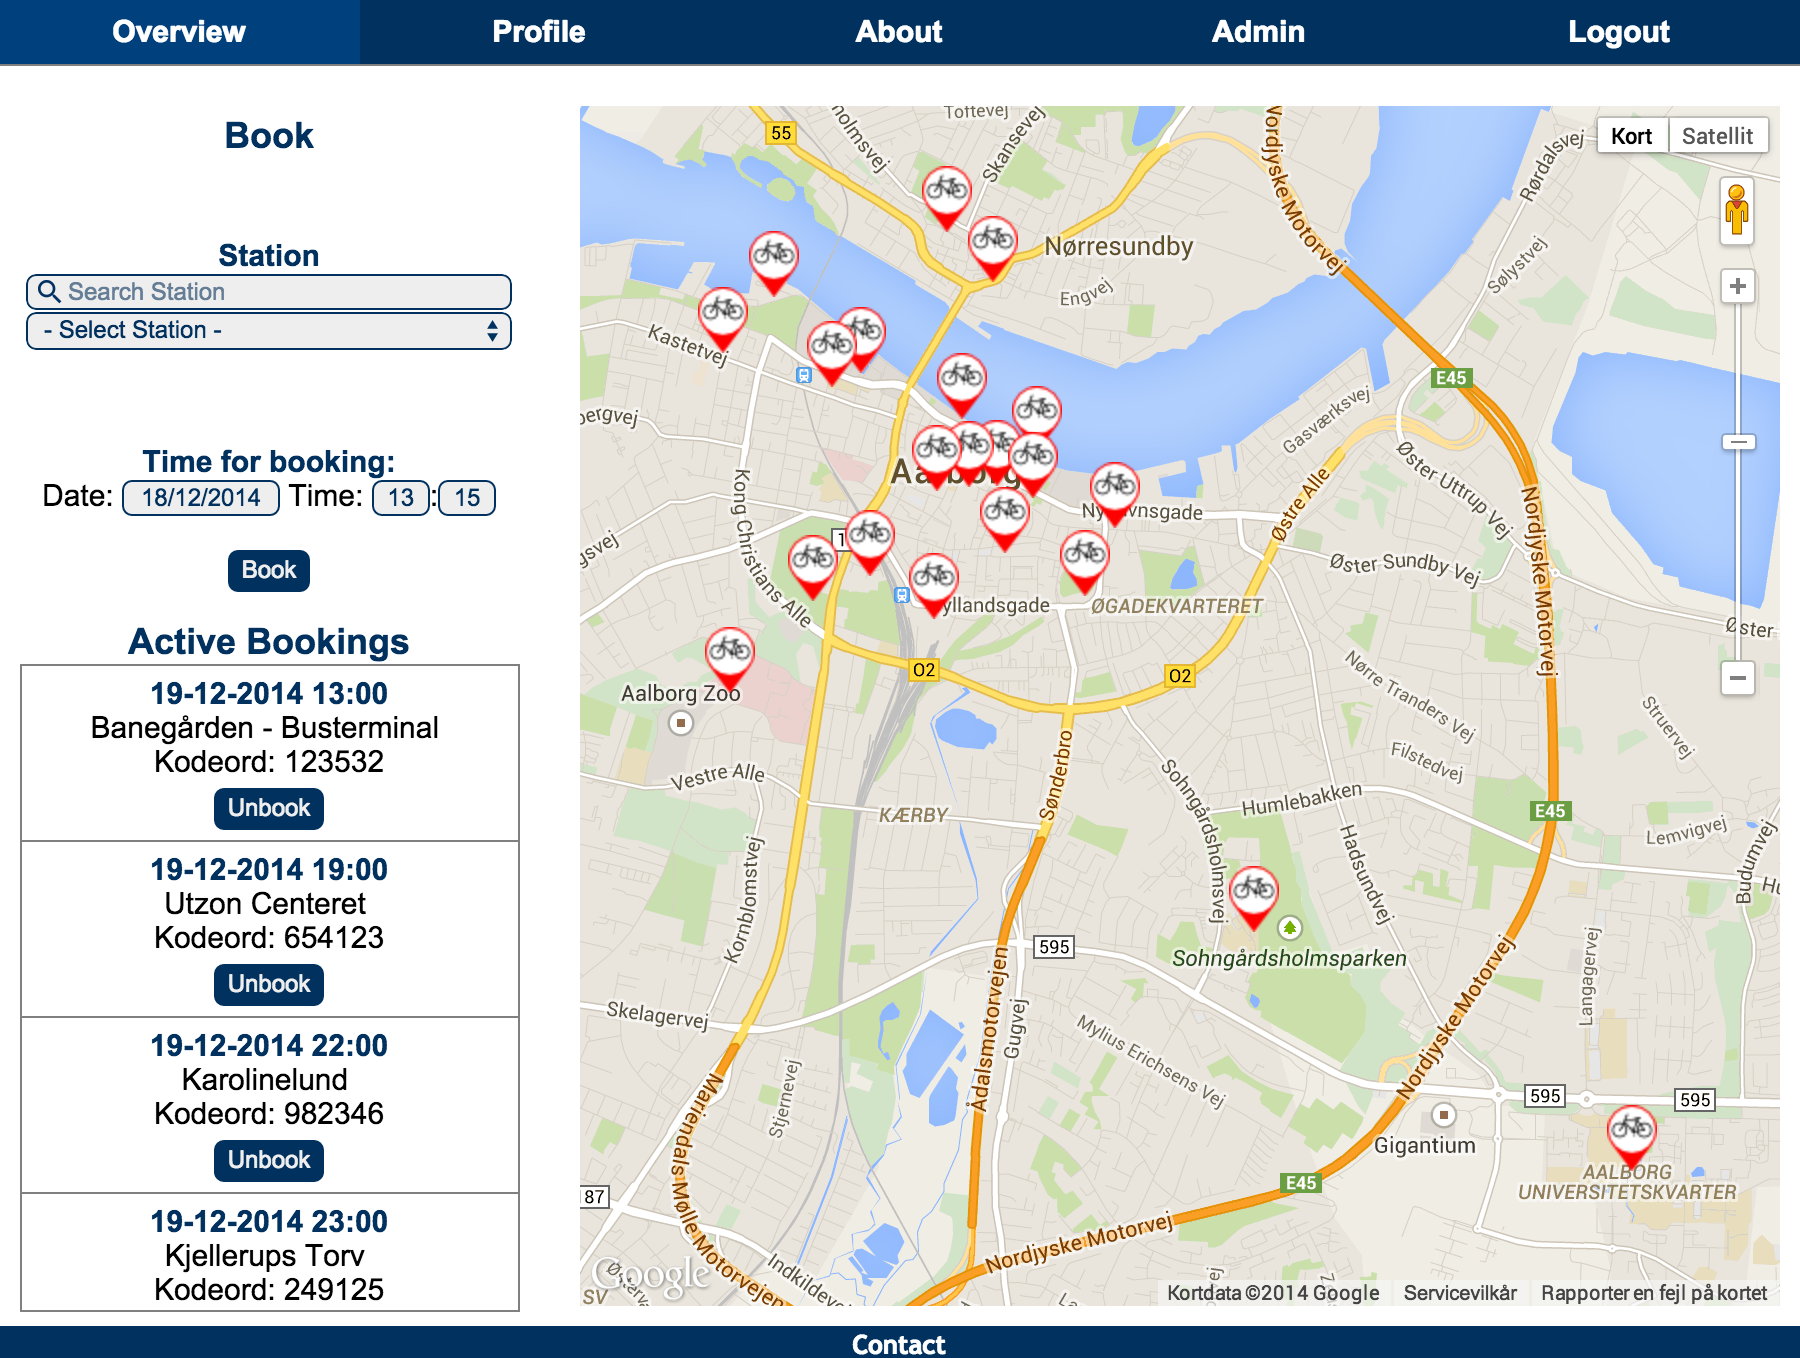
\includegraphics[scale=0.6]{UI/overview}
	\caption{Overview page}\label{fig:UI-overview}
\end{figure}

In this figure we can see that something from the prototype has been changed, mainly the fact that the screen is now only split in two parts, where the map showing station locations covers two thirds, and the bookings/station details cover the last third.
The map in the figure shows a map of Aalborg city with bicycle icons on it representing the station placements.
The right side of the website is used for booking, where users can book a bicycle on a chosen station at a specified time.
Pressing the book button creates a booking at the currently selected station and specified time.
The user can also see a list of bookings he/she currently has, and is able to cancel said bookings by clicking on the unbook button.

In \figref{fig:UI-overview} the header contains five elements, of which the admin element is only shown to admin users and directs the user to the admin section of the site when clicked.
The profile element in the header directs the user to their profile page, where they can change their profile information if so desired, as well as view the history of their usage of the system.


The admin features are created for use by Aalborg Kommune, and they start on the page that can be seen in \figref{fig:UI-admin}.
This page is almost just a map, however, the black dots on the map are used to represent the current position of bicycles.
The header can be used to navigate to the various admin tools, elaborated more in \secref{sec:impAdminTools}.
The only header element that does not direct to another admin site, is the home element, which sends the user to the overview page.
Additionally, if an ordinary user tries to access an admin page, via. the url, he will be redirected to the homepage.

\begin{figure}[h]
	\centering
	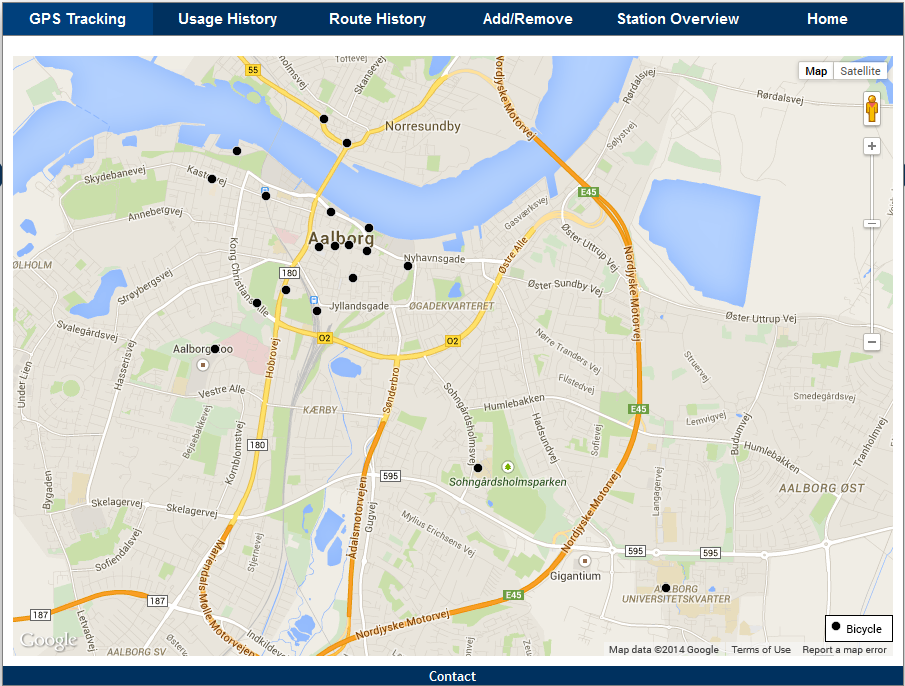
\includegraphics[scale=0.6]{UI/tracking}
	\caption{Admin page}\label{fig:UI-admin}
\end{figure}

	\section{Website Structure}
The website is structured via a modified MVC pattern, for an explanation of the general idea of MVC see \secref{sec:mvc}.
In order to make the usage of MVC smooth, a framework was used \citep{misc:mvc-framework}.

The framework provides a controller base class that the new controllers inherit from, mainly providing a database instance.
It also provides an 'Application´ class that handles url parsing and navigation to the correct pages based on the url.
In addition to this, it provides a directory structure. As an example, you can add a controller to the controller directory, and the 'Application´ class is able to load them, same idea goes for the model and view layer.

\begin{figure}
	\centering
	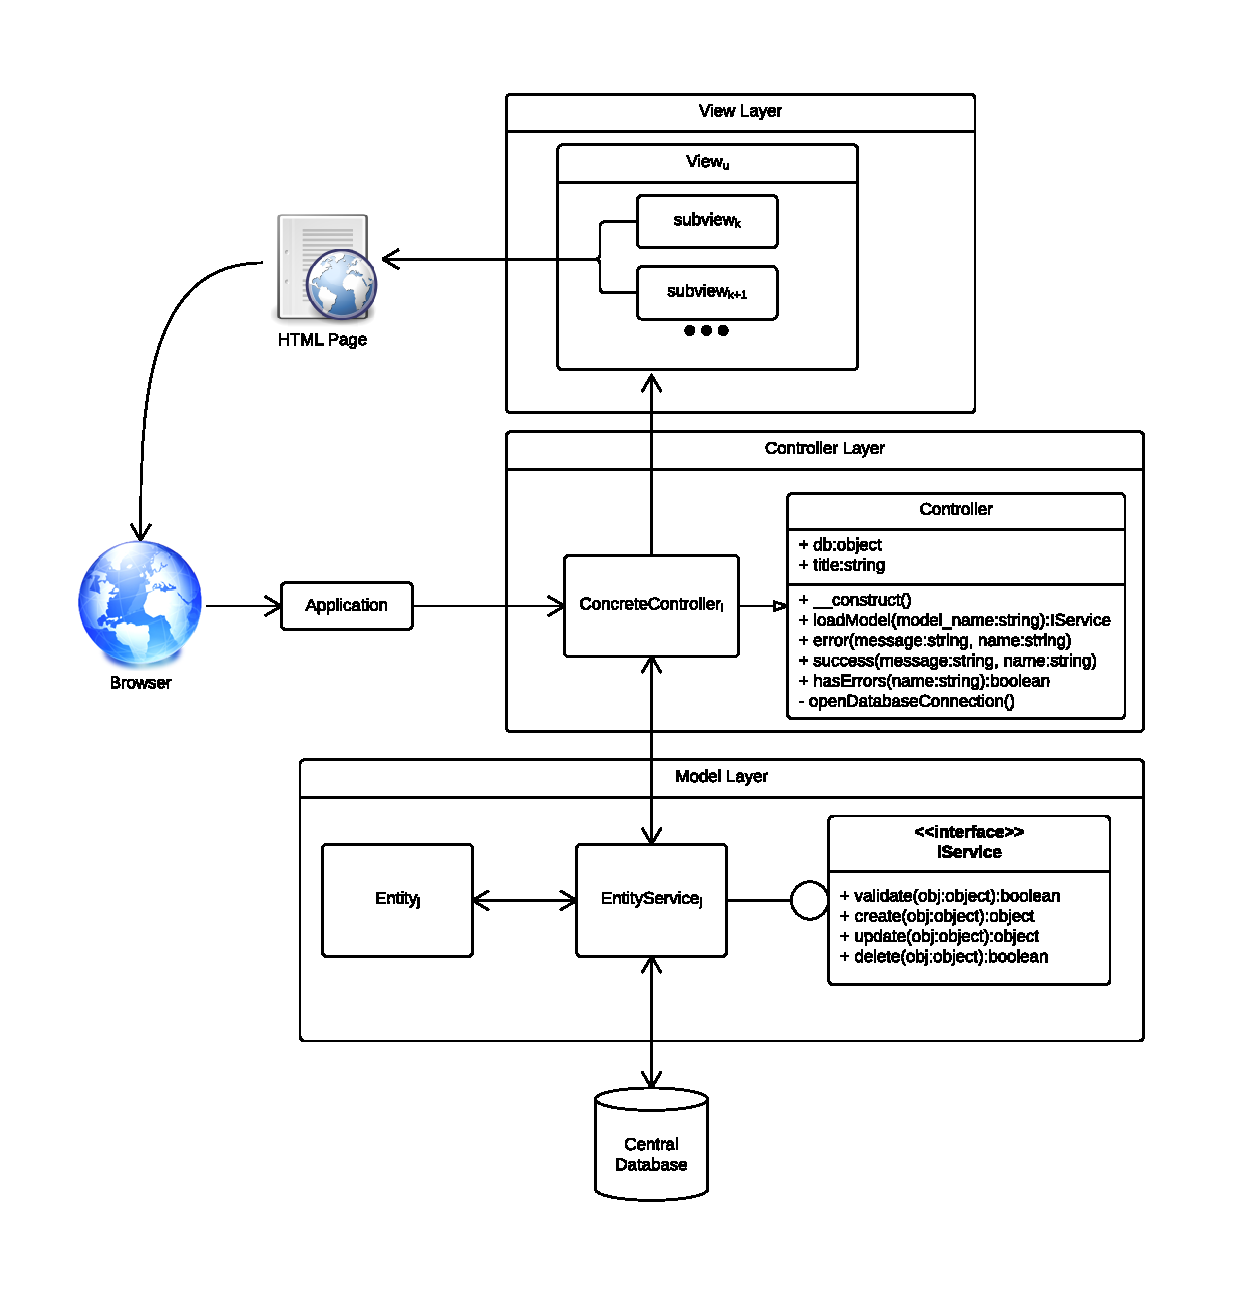
\includegraphics[scale=0.7, trim= 1cm 1.5cm 1.5cm 1.5cm, clip]{implementation/ConcreteMVC}
	\caption{Website Structure}\label{fig:websitestructure}
\end{figure}

With inspiration from the MVC pattern and usage of the framework, the website was then structured as seen in \figref{fig:websitestructure}.
The idea of the figure is to represent the structure, where we abstract from concrete entity, view, and controller names, and instead denote these with the names '$\text{Entity}_\text{j}$´, '$\text{EntityService}_\text{j}$´, '$\text{ConcreteController}_\text{i}$´, '$\text{View}_\text{u}$´.
The structure is split into several parts, each of which is examined in turn. 

\begin{description}[style=nextline]
	\item[Model Layer] 
	If you take a look at the model layer, it is split into three parts, $\text{Entity}_\text{j}$, $\text{EntityService}_\text{j}$ and iService.
	$\text{Entity}_\text{j}$ is a wrapper class, which is used to encapsulate a row from a table in the database.
	$\text{EntityService}_\text{j}$ is then a service, implementing the CRUD methods of iService, read is exluded from the interface because the parameters needed for read varies.
	$\text{EntityService}_\text{j}$ is what part of the model that then establishes the connection to the database, and enables the controller to work on the model, via calling the CRUD methods of the service, when a read method is called from a controller, an entity or a list of entities representing the row(s) is then what is returned.
	The reason we differentiate between  $\text{Entity}_\text{j}$ and $\text{EntityService}_\text{j}$ is that we found it makes sense to differentiate between the data and the methods working on the data, this is due to the EntityService sometimes requiring multiple types of Entities. 
    Furthermore it provides a separation of responsibility from the Entities and the EntityServices, given that Entities only provide a means of representing a row in the database and that EntityServices provide the behaviour for those representations.
	
	\item[Controller Layer]
	The controller layer consists of a number of controllers $\text{ConcreteController}_\text{i}$, each of which inherits from a base Controller class, which provides functionality to load the model as well as registering successes and errors to be displayed to the user by the view(s).
	Each concrete controller then contains a number of functions, corresponding to different sites, these functions are also called 'actions´. 
    The responsibility of the concrete controller is then to work on the model and include views. 
	
	\item[View Layer]
	The view layer takes care of the HTML generation part of the website, for each view included by the controllers, it consists of a number of subviews.
	Complete views should be thought as a combination of subviews, where some subviews occur in different views.
    Different classes of subviews exist, normal subviews and templates that are used almost universally throughout the site, for example the header and footer subviews.
	The combination of these subviews, the complete view, then takes care of representing a HTML page to be provided to the browser.
	
	\item[Application]
	When the browser visits the website, rewrite rules has been set in the \textit{.htaccess} file, to ensure that the relative path part of the url is given as an argument to the default index file. This index file then loads the required files, such that the instantiated Application object has access to the configuration files needed.
	The GET variable url, which was set from the .htaccess file is then used by the Application object to navigate to the correct controller.
	
	
\end{description}

For a more detailed look at the model and controller layer, see \appref{app-arch:controller} and \appref{app-arch:model}.
	\section{Database}
To support the necessary information storage, a database is implemented in accordance with the ER diagram described in \secref{sec:ERdiagram}.
The implementation of the ER diagram leads to the database schema that can be seen in \figref{fig:Database-tables}, however, there is more than what the ER diagram describes.
In this figure, the connections between the tables represents foreign key constraints.

\begin{figure}[h]
	\centering
	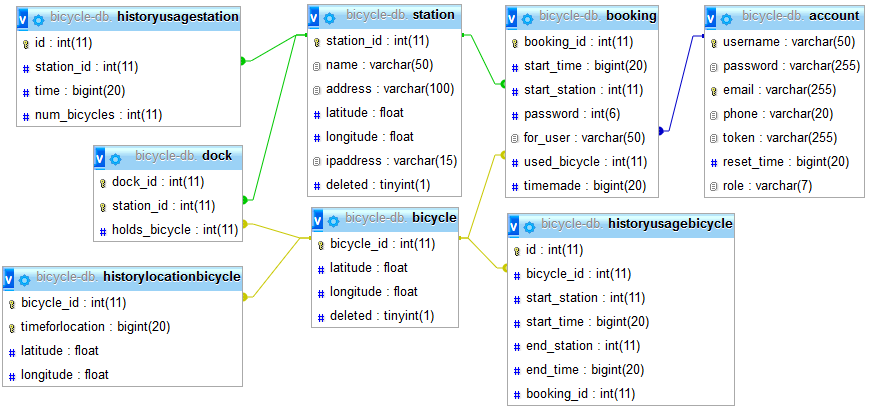
\includegraphics[scale=0.6]{Database/DBtables}
	\caption{Database tables}\label{fig:Database-tables}
\end{figure}

The additional tables (historyusagestation, historyusagebicycle, and historylocationbicycle) are added to store the information needed for the features described in \secref{sec:designAdminTools} and which implementation is discussed in \secref{sec:impAdminTools}.
The three additional tables serves as a log, in order to store information about usage of the system, to be used by the administration part of the system to analyse on the usage of the system.

Because of how logging is used is different from the general usage of the system because it has to use all historical data.
That means that for the purposes of the tables mentioned above it is important that for the station and bicycle tables that rows are not deleted, but rather just flagged as deleted, why is the cause of the deleted attribute in those tables. 
For regular use of the system it changes little but administratively it allows for using historical data.

In the translation from the ER diagram to the schema presented, the relations between the various entities could in all cases be represented as an attribute on one of the involved entities.
This attribute is a foreign key.
This was all that was needed to convert the ER diagram into the database schema, however, with the introduction of the administrator features and their associated data tables, more was needed.

When the administrator features was added into the database, in addition to adding three new tables to contain their information.
The administrator features also required addition of additional attributes to some of the already existing tables, an example of this being \textit{role} attribute on the account table, used to distinguish regular users from the ones with administrator privileges.

This was implemented in MySQL, primarily because it was packaged with the webserver that we used to develop the system with.
There is no reason why MySQL was chosen instead of competing DBMS such as postgresql or MSSQL other than convenience, and little reason why the schema could not be adapted to work on others.
	\section{Interfaces}\label{sec:interfaces}
As is described in the design, some communication between the stations and the database has to be established, to retrieve bookings etc.
This communication is established through the three interfaces gpsregister, websitetostationnotifier and stationtodbregister.
These interfaces being from website to station, station to database, and bicycle to database.
Each of these interfaces are described below.

\subsection{Website to Station}\label{sec:webToStationI}
This section is about the websitetostationnotifier interface from \figref{fig:overallarch}.
The website has to establish contact to a station when a booking or un-booking has been performed.
It is evident that this is important, as the stations need to be notified to keep track of bookings involving themselves as station.

This contact is established through TCP/IP, and is used in implemented notification methods.
These being \texttt{notifyStationDockChanged}, \texttt{notifyStationBooking} and \texttt{notifyStationUnbooking}.
The call to the notification methods is added in the \textit{BookingService}, as each time a booking is created, updated, or deleted, it is called through BookingService, and as of such we ensure the notification method is always called.

In general, the notification methods work in the following way:
\begin{itemize}
	\item Construct JSON encoded message to be sent to the station.
	\item Create the TCP socket.
	\item Connect the socket to the station involved with the booking.
	\item Send the data to the station.
	\item Close the socket.
\end{itemize}

The reason the message is JSON encoded, is to have a standard way of encoding data, which can be easily decoded by the station.
It is then up to the station to parse this information and perform the action specified in the message.
How the JSON encoded message looks like, as well as how the station handles this notification is elaborated in \secref{subsubsec:listener}.

\subsection{Station to Database}
This section is about the stationtodbregister interface from \figref{fig:overallarch}.
The station to database interface is important in order to register when a bicycle has been taken at a station or returned to a station, in order to give correct information on the website status page.
Additionally the interface is used to retrieve information about bookings registered in the large database, in case of power-up of a given station.

The interface has been implemented in a SOAP encoding by help of the NuSOAP library.\fxwarning{kilde her}
This library makes you able to write regular PHP functions and then register these with the NuSOAP library, in order to have a webservice generated.
Bear in mind that all methods registered with NuSOAP needs to have a return value and as such a dummy boolean value is used where no other return value is needed.

An example of the implementation of an update and read operation on the database is presented below.

\begin{minipage}{\textwidth}
\begin{lstlisting}[caption = {Method for registering a bicycle as been returned to a dock at a given station.}, label = {lst:bicycledockstationreturned}]
$server->register('BicycleReturnedToDockAtStation',
	array('bicycle_id' => 'xsd:int',
	'station_id' => 'xsd:int',
	'dock_id'    => 'xsd:int'),
	array('return' => 'xsd:boolean'),
	$SERVICE_NAMESPACE,
	$SERVICE_NAMESPACE . '#soapaction',
	'rpc',
	'literal',
	'Registers that a given bicycle has arrived at a given dock at a given station'
);
function BicycleReturnedToDockAtStation($bicycle_id, $station_id, $dock_id)
{
	global $db;
	$stmt = $db->prepare("UPDATE dock SET holds_bicycle = ? WHERE station_id = ? AND dock_id = ?");
	$stmt->bind_param("iii", $bicycle_id, $station_id, $dock_id);
	$stmt->execute();
	$stmt->close();
	
	[...]
	return true;
}
\end{lstlisting}
\end{minipage}

If you take a look at \lstref{lst:bicycledockstationreturned}, the code is split into two parts, line 1-11 and line 12-21, which handles different parts of providing a method to register that a bicycle has returned to a dock at a given station.

Line 1-11 takes care of registering the PHP function, such that it can be included in the auto-generation of the SOAP encoded webservice.
As can be seen from this specification, we tell the NuSOAP library the name of the function to register on line 1.
Then line 2-4 specifies the input parameters, line 5 specifies the return value, and line 6-11 is less interesting parts which deals with how the method should be represented in SOAP.

Line 12-21 is the actual method for registering that a bicycle has been return to a dock at a given station.
This is performed with use of prepared statements, as can be seen in line 15-18, which is done to prevent MySQL injection.
As you can see, the actual statement expresses an update on the dock, such that the dock, where the bicycle has been placed, gets this information updated.

\begin{minipage}{\textwidth}
\begin{lstlisting}[caption = {Method for reading all bookings for a given station}, label = {lst:getallbookingstation}]
$server->register(
	'GetAllBookingsForStation',
	array('station_id' => 'xsd:int'),
	array('return' => 'tns:BookingObjectArray'),
	$SERVICE_NAMESPACE,
	$SERVICE_NAMESPACE . '#soapaction',
	'rpc',
	'encoded',
	'Get all bookings for station'
);
//in case you want to read everything.
function GetAllBookingsForStation($station_id)
{
	//returns all bookings from database from a given station, as a json encoded array.
}
\end{lstlisting}
\end{minipage}

An example of a method that reads from the database is the \textit{GetAllBookingsForStation} function, seen in \lstref{lst:getallbookingstation}.
Such a method is for example useful when first booting a station where its local database is empty or that the local database data is outdated, e.g. it has been offline for some time.

Taking a look at line 1-10, you see the registration of the PHP function for integration in the SOAP specification.
As can be seen, it utilised a custom type called \textit{BookingObjectArray}, which is an array type used to contain multiple JSON encoded strings that represents bookings.
The result is a JSON encoded array and can be used by the given station to traverse the array returned and decode each string to get its corresponding booking information.

\subsection{Bicycle to Database}
This section is about the gpsregister interface from \figref{fig:overallarch}.
The interface from bicycle to database, is an interface that is needed to register the location of a bicycle, as GPS tracking is decided to be implemented, due to the meeting held with Aalborg Kommune.
The idea is that each bicycle use the interface to inform the system where it is located, according to the coordinates received from GPS.

The interface is implemented in the same fashion as the interface from station to database.
As such, it is implemented as a SOAP web-service, using the NuSOAP library to gain the an encoding that makes the interface easy to call.
There exists one method, the \textit{RegisterGPS} method, which takes three arguments, the bicycle-id, latitude, and longitude.
The way this interface is constructed is similar to the other SOAP encoded interface, but where the bicycle location is updated instead.
	%!TEX root = ../../main.tex
\subsection{Model \& Model Services}
This section describe the implementation of the model layer. 
We illustrate this by giving an example model, showing what it looks like and what it does.
A diagram of the model layer can be seen in \appref{app-arch:model}.

The \texttt{Bicycle} entity class can be seen in \lstref{lst:bicycleModel}.
As can be seen, what it does is to capture the attributes of the Bicycle entity from the database.

\begin{minipage}{\textwidth}
\begin{lstlisting}[language=php, label=lst:bicycleModel, caption={Bicycle Class}]
<?php
class Bicycle
{
    public $bicycle_id = null;
    public $longitude = null;
    public $latitude = null;

    function __construct($bicycle_id, $latitude, $longitude){
        $this->bicycle_id = $bicycle_id;
        $this->longitude = $longitude;
        $this->latitude = $latitude;
    }
}
?>
\end{lstlisting}
\end{minipage}

Every entity have a corresponding service that contain the manipulation and handling of objects of the same type as its corresponding entity. 
Each model service implement an interface enforcing the class to implement methods such as \texttt{validate}, \texttt{create}, \texttt{update}, and \texttt{delete}, for an overview see \figref{fig:websitestructure}. 
Enforcing these methods to exist in every service dictates the responsibility of the service, for example enforcing a \texttt{validate} method dictates that it is the responsibility of the service to ensure a correct format of the model entity before making any changes to the database. 
Furthermore, CRUD dictates that the service should handle all contact with the database concerning its specific entity.

It is also the responsibility of the model to handle all reads from the database, although it is not included in the implemented interface.
This is because it may not always make sense to have a method that can read an entity from the database, and thereby this would possibly never be used.
The reason for this is because what you want to read varies a lot, e.g. do you want to \texttt{read} multiple rows from the database or a single row.
This is in contrast to \texttt{delete} or \texttt{update} that works on a single row.

With the model layer described, we take a look at how the controllers are constructed, and how they use the model layer.
	\section{Controller}
This section shows how the controller layer works. 
We illustrate this by giving an example controller, showing what it looks like and what it does.

In \lstref{lst:homeController} part of the Home Controller can be seen. 
It defines an `action', this action is what is interpreted from the request sent by the client. 
For space saving purposes all actions but the index action have been omitted.
The home controller uses two services, StationService, used to retrieve an array of all stations, line 8-9, and BookingService, used to retrieve an array of all active bookings for the currently logged in user, line 11-14. 
This illustrates the general idea behind the separation of the entities (the models) and the services associated with those entities.
It then uses the information loaded by `including' views, and these views then use this information for displaying the content read from the services.

\begin{lstlisting}[language=php, label=lst:homeController, caption={Home Controller Class}]
<?php
class Home extends Controller
{
    public function index()
    {
        $this->title = "Home";
        $currentPage = substr($_SERVER["REQUEST_URI"], 1);
        $stationService = new StationService($this->db);
        $stations = $stationService->readAllStations();

        if (Tools::isLoggedIn()) {
            $bookingService = new BookingService($this->db);
            $activeBookings = $bookingService->getActiveBookings($_SESSION["login_user"]);
        }

        require 'application/views/_templates/header.php';
        require 'application/views/home/index.php';
        require 'application/views/_templates/footer.php';
    }
    // [...]
}
\end{lstlisting}

As can be seen on line 16-18 three views is included into the function. Because of the way include works in PHP the included content is in the same scope as the rest of the function, which means we can use the variables declared in the function, inside the included content.

The controllers and their `actions' can be seen in \appref{app-arch:controller}.
	\section{Views}
This section will describe the view layer and what it does, illustrating by example. For more detail about Model-View-Controller architecture, see \secref{sec:mvc}.

In \lstref{lst:homeIndexView} a truncated version of the home index view can be seen. Most of it is normal HTML, but the important part is how it utilizes variables set in the controller, because a view included by the controller gives it access to its variables. This allows it to use them to generate more HTML as can be seen lines 6--10 where it uses the array of stations set in the controller to output option elements in a select element, and it can also use methods defined as shown in line 13--19.

\begin{lstlisting}[language=html, label=lst:homeIndexView, caption={Home Index View}]
[...]
<form action="/Home/Book/" method="post">
    [...]
    <select name="station" id="stations" style="width: 243px;" onchange="UpdateMarker()">
    <option value="0" disabled selected>- Select Station -</option>
    <?php
    foreach($stations as $station){
        echo '<option value="'.$station->station_id.'">'.$station->name.'</option>';
    }
    ?>
    </select><br />
    [...]
    <?php
        if (Tools::isLoggedIn()){
            echo '<input type="submit" value="Book" />';
        } else {
            echo '<a href="/User/Login/">Login</a>';
        }
    ?>
    [...]
</form>
[...]
\end{lstlisting}

	\section{Google Maps API}\label{sec:googlemapsapi}
The Google Maps API \citep{misc:googlemapsapi} is used to show maps on the front page and some of the administration pages.
However, both of these pages use the API differently, the front page uses the API to show the map with the stations that are currently in the system, whereas the administrator page visualises where all the bicycles are located.

To use the API, the construction of the map is done first, which can be seen in \lstref{lst:mapoptions}.
Map options are chosen, these options are e.g. the center of the map, which zoom level the map should have, and the style of the map.

\begin{minipage}{\textwidth}
\begin{lstlisting}[caption={Construction of the map.}, label={lst:mapoptions}, language=Javascript]
var mapOptions = {
	zoom: 13,
	center: aalborg,
	panControl: false,
    zoomControlOptions: {
		style: google.maps.ZoomControlStyle.LARGE,
		position: google.maps.ControlPosition.RIGHT_TOP,
	}
};
\end{lstlisting}
\end{minipage}

After the map is constructed the map is filled with either the stations or the bicycles, depending on the page.

For the front page the stations are inserted into the map by use of AJAX.
For each station, the work-flow of this is as follows:

\begin{description}[style=nextline]
	\item[Gather data]
	Use the station service to read data to be displayed on the map.
	\item[Create info window]
	The info window is a window that appears whenever the user clicks on a station marker.
	It shows information about the station, which is the name, amount of free bicycles, and the amount of free docks.
	\item[Marker creation]
	Create a marker, which are the bullet points indicating the station on the map.
	The creation of the marker contains position, title, icon.
	\item[Assign listeners]
	Assign listeners to the marker clicks, in order to show the info window for the given marker when the marker is clicked.
\end{description}

\begin{figure}[h]
	\centering
	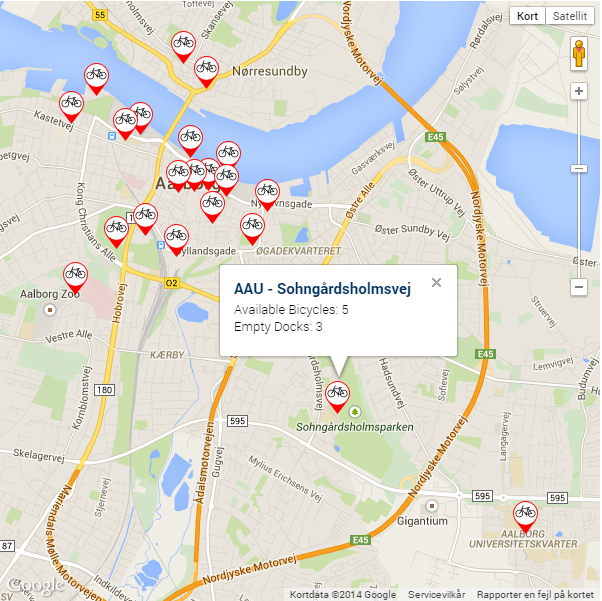
\includegraphics[scale=0.7]{googlemarkermap}
	\caption{Google map with station markers and info window shown.}
	\label{fig:googlemapmarkerinfowindow}
\end{figure}

An example of the final Google map with markers placed can be seen in \figref{fig:googlemapmarkerinfowindow}.

For the administrator page the markers are bicycles, which are updated at a set frequency using AJAX, and is created in a similar fashion, but with other objects placed on the map.
The main purpose of the administrator tracking page is to be able to see where the different bicycles are at a given time, which is the reason why the markers are updated once in a while.
For the update of the marker position AJAX is used to get all the positions of the different bicycles, which allows the makers to move without refreshing the page.
	%!TEX root = ../../main.tex
\section{Administration Tools}\label{sec:impAdminTools}
% This section describes the administrative functionality. 
% It covers route history, GPS history, bicycle usage history, and an add/remove page.
% It also contains a bicycle GPS tracking, but this has been mentioned in \secref{sec:googlemapsapi}.
In \secref{sec:designAdminTools} some questions were asked. 
In this section we answer these questions.
To answer the question about which routes are used we implemented a feature to show route history, which can be seen in \secref{sec:routeHistory}.
Hotspot detection was not implemented, but GPS history was implemented in \secref{sec:gpsHistory}.
The traffic og bicycles during some period and the current amount of bicycles at a given station can be seen using the implemented graph in \secref{sec:bicycleUsageHistory}.
How the amount of bicycles at a station change over time can be seen in the same graph.

%We also implemented a page for addition and removal of users, bicycles, and stations.


\subsection{Route History}\label{sec:routeHistory}
This part of the administration site handles showing a map of the historical locations of a bicycle.
The admin provides one or more bicycles, a start, and end date.
Then if there are historical GPS coordinates for the bicycle(s), they will be shown on the map. 

The purpose of the route history page is to give the admins an idea of which roads the bicycles are traveling a lot on. 
This can then be used as a decision-making tool to decide where to put new stations, in that if the admin can see that a lot of bicycles are traveling to a specific point it might be a good idea to put a station there.
It could also be used to see if a specific bicycle is being 'misused' in the sense that it would be visible if the bicycle is only being used to travel to one spot and nowhere else.

See \figref{fig:routehistory} for a figure of what the page looks like.

\begin{figure}[H]
	\centering
	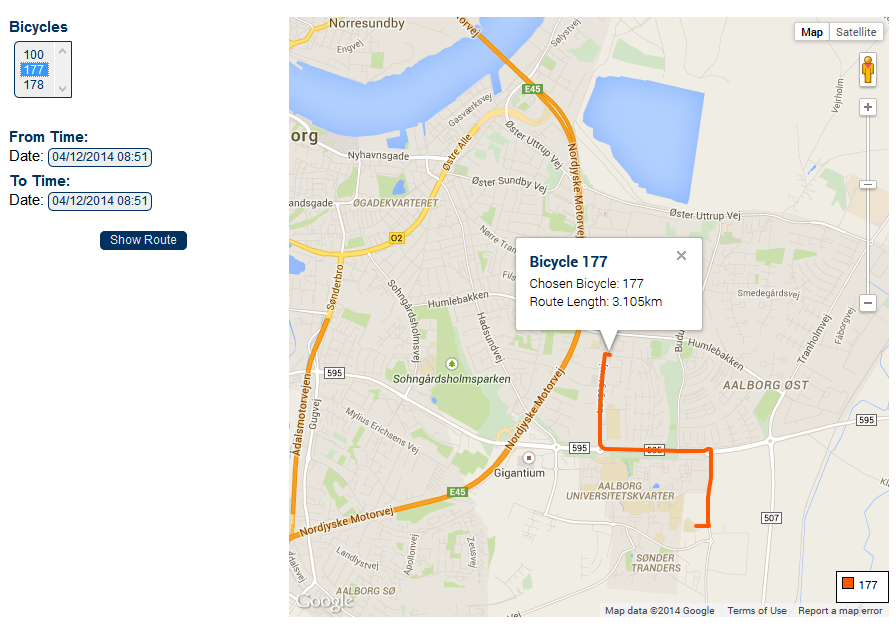
\includegraphics[scale=0.75]{RouteHistory.png}
	\caption{Picture of Route History}
	\label{fig:routehistory}
\end{figure}

It is implemented by finding all the bicycles that have associated historical GPS data.
 The administrator then chooses which bicycles to map, and these bicycles then have their routes loaded which are then given to Google Maps API to display.


\subsection{GPS History}\label{sec:gpsHistory}
The system saves the location of bicycles registered in the system, which could be helpful for determining where bicycles currently are. 
This would allow the 'county' to determine where 'lost' bicycles are, which in turn would allow for easier recovery of bicycles.
Having the GPS tracking already implemented, it makes sense to store the GPS coordinates in a separate table for historical and business intelligence purposes.
This kind of historical data could be interesting for intelligence purposes because it would allow knowledge about the following:

\begin{description}[style=nextline]
\item[Which routes are used?] If routes could be determined, patterns could possibly be seen, e.g. if there is a particular route that is very popular.
\item[Are there hotspots for bicycles?] If positions of bicycles could be determined, it would mean that hotspots(places where there is a lot of bicycle activity) could be found. 
This could provide valuable knowledge about for example where to add new stations.
\end{description}

A table to store this is created, containing the following information:

\begin{itemize}
\item The ID of the Bicycle
\item A timestamp of when the coordinates was recorded.
\item The latitude and the longitude.
\end{itemize}

At the same time when location is recorded from a service, it needs to also record it permanently in the global database.

\subsection{Bicycle Usage History}\label{sec:bicycleUsageHistory}
% Disposition:
% What does it track?
% Which questions can be answered?
% How is it implemented?

Besides recording the exact location of each bicycle with GPS coordinates, the system also records the stations a given bicycle visits. 
This can be used to give an overview of the bicycle traffic between stations.
Furthermore, the amount of docked bicycles is tracked for each station, giving an overview of which stations that have high and low activity.

\begin{description}[style=nextline]
\item[Where is the most traffic of bicycles during some period?] An admin user would be able to see how many bicycles leaves and arrives at each station and thereby get an overview of where the traffic is high and low, providing an indication of where to put focus for relocation of bicycles and expansion of stations.
\item[What is the current amount of bicycles at a given station?] A graph is shown providing the amount of bicycles on the y-axis and the provided timespan on the x-axis. This gives the admin user an idea when bicycles leave each station.
\item[How does the amount of bicycles at a given station change over time?] Taking the same graph as above, the admin user can also choose a long period of time for example a week, month or a year, providing a more general overview of when the activity at each station is high or low.
\end{description}

These features are implemented through two additional tables added to the database, where the first table keeps information about the amount of bicycles at a station along with a timestamp. 
The other table keeps information about the time and station a bicycle left from and arrived to, along with the specific bicycle id and a possible booking id associated with the bicycle trip.

As this information needs to be captured and updated when an event occurs, either being a bicycle that is taken from a station dock or a bicycle return to a station dock, these operations are performed in the interface between the stations and the global database, see \figref{fig:overallarch}. 
The stations will communicate with this interface when either of these events occur. 
The timestamp is generated just before query execution, which means that some delay can occur from the actual event firing time to the insertion time, resulting in an imprecise trip duration. 
This is, however, considered a minor deviation in most cases, because the communication delay is short (seconds maybe even less).
In case of a bad connection, the generated timestamp will cause useless data in the light of statistical usage, if time is an important aspect of the analysis.
For showing the traffic between stations the timestamp is used for filtering on a specified time interval and thereby allowing up to an hour of imprecision.
This time interval is an assumed granularity and would have to be specified by the admin.
The graph showing the amount of bicycles docked at a station shows the timestamp on the x-axis, however, in this case it is considered acceptable with some imprecision since this data will not be used for statistics but for a visual overview.
	%!TEX root = ../../main.tex
\section{Station Software}
The station software package contains two aspects, software intended to be run on the stations that are placed at each station location throughout the city, and software to simulate the hardware we do not have access to, used as proof of concept.
For an overview of the station structure, see \figref{fig:stationarch}. 
However, to use these two aspects a graphical user interface is needed, and is described hereafter.

\subsection{User Interface}
The Main UI window has two parts, which can be seen in \figref{fig:stationMain}, part one is the station software, and part two is for the hardware simulation, which is explained later in this section.

\begin{figure}[h]
	\centering
	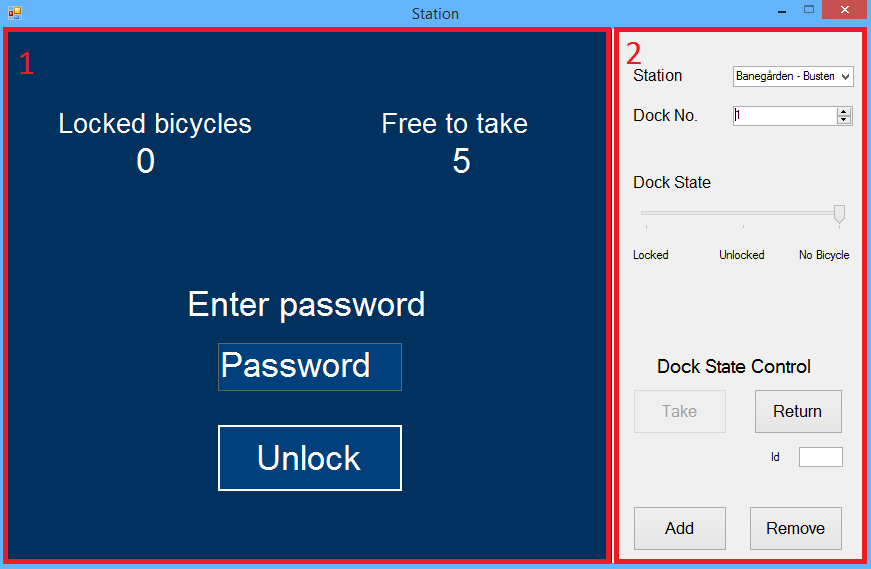
\includegraphics[scale=0.4]{stationsoftware/mainwindow}
	\caption{UI for the station software}\label{fig:stationMain}
\end{figure}

The station software UI, part 1 in \figref{fig:stationMain}, has been designed to be simple and understandable by users of the system with only the necessary content.
The blue colour was chosen as this is the colour of the bicycles and the \bycykel website.
The station software UI is divided into two pages, the first one can be seen in the figure.
It has a field to input a password for a booking to unlock the booked bicycle.
In addition to this it also displays how many bicycles on the station that are locked and how many that are free to take.
When a valid booking password is input, the station UI changes to the other page, which can be seen in \figref{fig:bicycleUnlock}.
The user is told at which dock the bicycle for him has been unlocked.
There is also a button to quickly return to the main window, which otherwise happens after 10 seconds.

\begin{figure}[h]
	\centering
	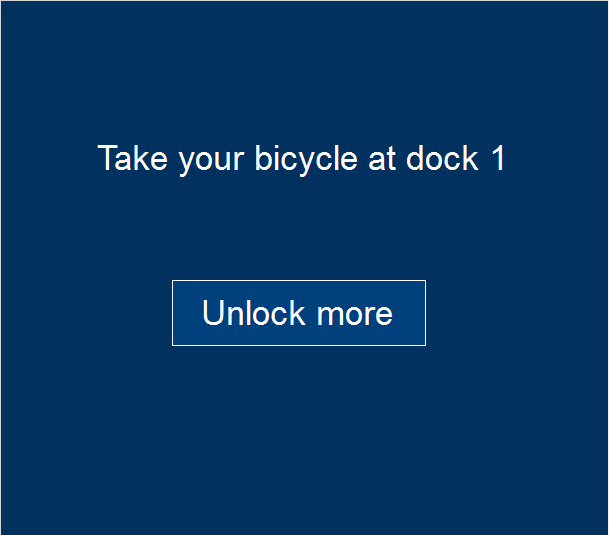
\includegraphics[scale=0.4]{stationsoftware/unlockwindow}
	\caption{UI for unlocked bicycle}\label{fig:bicycleUnlock}
\end{figure}

\subsection{Station Backend}
The station backend contains three responsibilities as listed below, see \secref{subsec:stationsoftdesfgi}.
\begin{itemize}
	\item A listener that listens for signals from the global database interface called \texttt{WebsiteTo\-StationNotifier}, see \secref{sec:webToStationI}, signalling that a booking has been created or removed.
	\item A lock manager that is responsible for locking a bicycle at a dock when a booking is close to its start time, and unlocking if a booking has expired.
	\item Communication with the global database through a SOAP service interface described in \secref{sec:stationToWebI}.
\end{itemize}

In the following each of these three responsibilities are described further.

\subsubsection{Listener}\label{subsubsec:listener}
The listener is made as a TCP Listener based on code found on Microsofts Developer Network \citep{misc:TcpListenerSource}. 
The listener listens for messages, which is done on port 10000, reporting changes in bookings, either addition or removal of one. 
The messages are JSON encoded strings of different forms depending on the content, two such examples can be seen in \lstref{lst:JsonUnbooking} and \lstref{lst:JsonBooking}.

\begin{minipage}{\textwidth}
\begin{minipage}{0.45\textwidth}
\begin{lstlisting}[caption = {Example of an unbooking message}, label = {lst:JsonUnbooking}, language=TeX]
{
 "action":"unbooking",
 "start_station":5,
 "booking_id":2
}
\end{lstlisting}
\end{minipage}
\hspace{0.5cm}
\begin{minipage}{0.45\textwidth}
\begin{lstlisting}[caption = {Example of a booking message}, label = {lst:JsonBooking}, language=TeX]
{
 "action":"booking",
 "start_station":5,
 "booking_id":2,
 "start_time":1414135298,
 "password":483923
}
\end{lstlisting}
\end{minipage}
\end{minipage}

The information contained in the received message is then used to either remove a booking from the database, or add a booking to the database at the specified station, which action to perform is decided based on the action parameter.

\subsubsection{SOAP Service}
%-communication with global DB
The SOAP Service is used to report changes in the local data of the station to the global database, which is implemented in the \texttt{StationToDBRegister} interface, see \secref{sec:stationToWebI}.
The methods in use along with at description of when they are used is listed below.

\begin{description}[style=nextline]
\item[BicycleWithBookingUnlocked] Used when a booking has been used by the user and when a booking has not yet been used but has expired.
\item[BicycleTaken] Used when a bicycle has been taken at a dock possible by means of a booking.
\item[BicycleReturnedToDockAtStation] Used when a bicycle has been returned to a dock.
\item[SyncDockStatus] Used when a dock has been added or removed from a station. It synchronises the status of the docks at that station.
\end{description}

At the start-up or reboot of a station all bookings are synchronised, in order to get updated information for that station, where all bookings are first removed from the station database, and then all bookings are requested from the global database through the interface, using the method \texttt{GetAllBookingsForStation}.
This is done in order to have up to date information and catch bookings performed while the station was offline.

With the communication between the station software and the global database, there is a risk of losing data during the communication or not having a connection at all.
However, this connection loss is taken care of by starting threads that attempt to send the data to the global database every second.
This do give another problem which is when the threads are executed, which does matter because if a bicycle is returned and taken shortly after, the threads can be executed in a different order which makes the system believe that the bicycle is at the station. 
In order to solve this, a queue of function calls are made, so that the function calls are called in the right order, and thereby making this part of the program thread safe.
In other words, the function calls are serialised.
\subsubsection{Lock Manager}
The \textit{LockManager} runs in its own thread, with the sole responsibility of locking and unlocking docks based on booking start times. 
Currently the time constraints is set to locking a bicycle to a dock one hour before booking start time, and unlocking again one hour after start time, see \secref{subsec:lockingcons}. 
As this functionality requires constant monitoring, the function is run in an infinite thread, however, since we do not want to waste our processor time by executing this constantly, it sleeps for a short period of time after each iteration.

The loop starts out by finding all the expired bookings, removing the lock they had on a bicycle, telling the global database that the bookings have expired, and removing the bookings from the station database.
The loop then finds all bookings that start within the next hour and locks a bicycle for each booking not locked in the last iteration of the loop, if possible. 
It is important to note that if more than one booking start at the same time, the order of docks being locked is given by when the booking was created. 

At the end of the execution of the loop the UI is updated to reflect any changes performed to the database.

\subsection{Simulation of Hardware}
The part of the UI representing the simulated hardware is the second part seen in \figref{fig:stationMain}.
The simulated hardware represents what would normally be observed at the physical station.
We simulate the ID chips on the bicycles and the lock on the dock.
The ID chips are simulated when they would normally have been read at the docks, which is when the bicycles are returned to it after use.
In this case, when a bicycle is returned, we find a random ID from among those not currently in a dock, and selects this as the ID returned.
Random ID is sufficient at this time, as we have no way of predicting where a bicycle in use would be returned to.
Alternatively a bicycle ID can be specified from the GUI, giving more control for illustration purposes.
But for a real station, this can be performed with an RFID chip.
The lock is simulated by a boolean representation, stating if it is locked or not.

In the simulation part of the UI, there is a dropdown list where it is possible to select which station a user is standing at, along with a numeric selector allowing selection of a specific dock at the current station.
In addition, there is also a slide bar showing the state of the selected dock.
The possible states being locked, unlocked, and no bicycle.
At the bottom of the UI there are four buttons that simulate the user actions of returning and removing a bicycle, a field giving the option of specifying which bicycle is returned, and buttons to add and remove docks at the selected station.

For the addition and removal of docks it is handled station-side and not centrally, because otherwise it would require the administrator to add the dock to the system on the website and it could create situations where the administrator adds a dock that does not exist at the station.  
This is of course a design choice that could work in either direction, but due to the reasons given station-side seemed more natural.
	\section{Synchronisation}
As the system is split into stations and a central system, it is necessary to have communication between them, and tackle the synchronisation of data.
This communication data flow have been illustrated in \figref{fig:overallarch}, additionally see \secref{sec:sync} has discussed this problem previously as well.

\begin{description}[style=nextline]
	\item[Bicycle locking/unlocking not synchronised]
	What is important for the central part of the system to know is at what docks at stations bicycles are placed.
	However, it is not important for the central system to keep track on what bicycles are locked and unlocked at a station, as this information is of no use for the central system.
	The information is on the other hand important for the station, as this is the part of the system that ensures that bicycles are locked in time.
	For that reason, the information is kept at the station. Furthermore, the central system can calculate how many bicycles are locked at a given station, as it can use the bookings for this.
	
	\item[Removal/Insertion of bicycles]
	On the other hand it is important for the central system to know when a bicycle has been removed or inserted at a station.
	This is due to the website providing status information to the user, such that they can know where free bicycles are located.
	The communication to ensure this, as previously mentioned, is then performed by use of SOAP.
	In order to ensure that this communication goes through, the station has a seperate thread to communicate this information, if the station is unable to communicate that a bicycle has been removed/inserted, it will wait a bit and then try again until connection has been established.
	
	\item[Booking/Unbooking]
	The booking and unbooking of bicycles are performed on the website. 
	The central database is then updated accordingly, and in order to ensure that the station affected is notified, a TCP package is sent, which contains the JSON encoded action, as described earlier.
	However, problems may arise if the connection to the station is down.
	In such a case, you can risk the station not registering the booking, and as of such, one of the following actions have to be performed.
	\begin{itemize}
		\item Flag to indicate new bookings
		\item Constantly ping central database (unreliable)
		\item Call local service to continuously try and connect until notification has been achieved.
		\item Give the user an error message, telling him to try and book/unbook again later. 
	\end{itemize}
	
	The idea behind having a flag to indicate new bookings is that a flag will be set for the station that failed to be connected to.
	On the station side, a thread will then run and check every $x$ amount of seconds for a flag that may have been sent.
	If such a flag is registered, the station then knows that it should update its bookings to correspond to those of the central database.
	
	Another more simple, but non reliable, idea is to constantly ping the central database.
	If you for one or several of your pings then fail to connect to the central system, you know that the next time you get connection, you have to update the bookings.
	One problem that makes us not use this approach, though, is in the timespan of two pings, if the connection fails there, the station will not get notified of a registered booking in that said time-period.
	
	Those two ideas involves giving the station the responsibility of having up to date booking information.
	However, another perspective can also be taken.
	One such approach is to develop a service to run on the central part of the system.
	The responsibility of this service is then to ensure that the station will get notified.
	The idea is that the service holds queues of notifications to be sent out, one such queue for each station.
	The service can then get notified to enqueue a notification, but the service will then continuously try and deliver the notifications from the queues to the stations. 
	This is found to be a good approach, since it ensures that when connection is established to a station again, the notifications it needs gets delivered.
	
	The last approach is to give the user an error message telling him to try and book/unbook again later.
	This approach is not desirable as we want the system to be as responsive as possible.
	The approach with a flag or the additional notification service is desirable.
	However, due to lack of time, it has been chosen as the solution, it was deemed a necessary compromise, but with more time, the flag or the separate service solution would be strived for.
	 
	
	\item[Station boot/reboot]
	When the station boots/reboots it may have missed some booking information.
	For that reason, when the station boots/reboots it reloads the booking information.
	However, with the notification securing set in place, this should not be necessary.
	This part of the synchronisation was developed before the other part, though, and is kept in case the other synchronisation techniques for some reason fails.
	Additionally, as this is a simulation, we run the station software on different computer, and as of such it is advantageous for testing to keep this updating of booking information in place, such that the various computers gets the booking information updated.
	
	\item[Dock insertion/removal]
	When a dock gets inserted or removed from a station, the station has a separate thread that keeps trying to call the web-service set in place on the central system part, to register that a dock has been inserted/removed at the given station, this is repeated until the web-service has been correctly used.
	This is achieved with specific functions set in place for the `stationtodbregister' service.
	
	\item[Hardware versus software simulation]
	For the system developed, software simulation of hardware has been used.
	However, if you were to implement real docking hardware, a synchronisation between the stations and its docks would have to be considered.
	This is somewhat achieved with the local database set for each station, however, with the sensors active, you would need to setup some communication protocol between the station and its docks, to ensure that the local database is up to date.
	Additionally, to go the other way around and send signals to the docks, notifying them if they should lock or unlock some bicycle.
	
\end{description}

This ends the general synchronisation implementation details, with a brief documentation of our testing following hereafter.
	%%!TEX root = ../../main.tex
\section{Usage History for Business Intelligence Purposes}
This section describes various usage history features that were implemented, and why. It includes the GPS History and Bicycle Usage History.

\subsection{GPS History}
The system saves the location of bicycles registered in the system, which could be helpful for determining where bicycles currently are. 
This would allow the 'county' to determine where 'lost' bicycles are, which in turn would allow for easier recovery of bicycles.
Having the GPS tracking already implemented, it makes sense to store the GPS coordinates in a separate table for historical and business intelligence purposes.
This kind of historical data could be interesting for intelligence purposes because it would allow knowledge about the following:

\begin{description}[style=nextline]
\item[Which routes are used?] If routes could be determined, patterns could possibly be seen, e.g. if there is a particular route that is very popular.
\item[Are there hotspots for bicycles?] If positions of bicycles could be determined, it would mean that hotspots(places where there is a lot of bicycle activity) could be found. 
This could provide valuable knowledge about for example where to add new stations.
\end{description}

A table to store this is created, containing the following information:

\begin{itemize}
\item The ID of the Bicycle
\item A timestamp of when the coordinates was recorded.
\item The latitude and the longitude.
\end{itemize}

At the same time when location is recorded from a service, it needs to also record it permanently in the global database.

\subsection{Bicycle Usage History}
% Disposition:
% What does it track?
% Which questions can be answered?
% How is it implemented?

Besides recording the exact location of each bicycle with GPS coordinates, the system also records the stations a given bicycle visits. 
This can be used to give an overview of the bicycle traffic between stations.
Furthermore, the amount of docked bicycles is tracked for each station, giving an overview of which stations that have high and low activity.

\begin{description}[style=nextline]
\item[Where is the most traffic of bicycles during some period?] An administrator would be able to see how many bicycles leaves and arrives at each station and thereby get an overview of where the traffic is high and low, providing an indication of where to put focus for relocation of bicycles and expansion of stations.
\item[What is the current amount of bicycles at a given station?] A graph is shown providing the amount of bicycles on the y-axis and the provided timespan on the x-axis. This gives the administrator an idea when bicycles leave each station.
\item[How does the amount of bicycles at a given station change over time?] Taking the same graph as above, the administrator can also choose a long period of time for example a week, month or a year, providing a more general overview of when the activity at each station is high or low.
\end{description}

These features are implemented through two additional tables added to the database, where the first table keeps information about the amount of bicycles at a station along with a timestamp. 
The other table keeps information about the time and station a bicycle left from and arrived to, along with the specific bicycle id and a possible booking id associated with the bicycle trip.

As this information needs to be captured and updated when an event occurs, either being a bicycle that is taken from a station dock or a bicycle return to a station dock, these operations are performed in the interface between the stations and the global database, see \figref{fig:overallarch}. 
The stations communicates with this interface when either of these events occur. 
The timestamp is generated just before query execution, which means that some delay can occur from the actual event firing time to the insertion time, resulting in an imprecise trip duration. 
This is, however, considered a minor deviation in most cases, because the communication delay is short (seconds maybe even less).
In case of a bad connection, the generated timestamp causes useless data in the light of statistical usage, if time is an important aspect of the analysis.
For showing the traffic between stations the timestamp is used for filtering on a specified time interval and thereby allowing up to an hour of imprecision.
This time interval is an assumed granularity and would have to be specified by the administrator.
The graph showing the amount of bicycles docked at a station shows the timestamp on the x-axis, however, in this case it is considered acceptable with some imprecision since this data is not be used for statistics but for a visual overview.
	
	\chapter{Test}
	In order to verify that the functionality of our system works as intended, we perform unit tests on our code. 
    To test the usability of our system, usability tests are also performed.
	\section{Unit Test}
Unit Tests are tests that are used to test the behaviour of the functions in a system.
When writing unit tests, the programmer sets up test cases and runs them through the function they are testing, and then compares the function output with the expected output.

As we have the source code of our program available, we have chosen the option of white-box testing.

The unit tests performed are performed on the model layer of the website aswell as the soap interface used to send messages to the station software.
As the tested parts are written in PHP, the PHPUnit testing framework is used for writing the tests. 
	\section{Usability Test}
This section covers the usability tests performed on the system.
Tests have been performed on the public part of the website, which are the status and booking.

These are the tasks:

\begin{description}[style=nextline]
\item[Task 1] Establish an overview
\item[Task 2] Status for bicycle
\item[Task 3] Booking - Login
\item[Task 4] Booking - Time and booking
\item[Task 5] Cancel planned booking
\item[Task 6] Examine the booking history
\end{description}
For a full description of the tasks see \appref{app:usability-test}.

The problems were uncovered using Instant Data Analysis.

The procedure for IDA is as follows:

\begin{itemize}
\item Test monitor introduces test subject to the evaluation procedure. After which the test monitor gives the first task to the test subject.
\item The test subject attempts to solve the task until they have accomplished it, feel they have accomplished it or until the test monitor gives them a new task.
\item Test subjects talk about what they are doing, explaining what they are doing and how they feel they understand the overall system. Test monitor does not help.
\item The test subject is interviewed and talk about their experience.
\end{itemize}\citep{misc:usabilitytest}

After the test, there is a meeting with the user where problems are discussed and which they felt were significant.
The result of Instant Data Analysis is a set of usability problems categorized into one of three categories: Critical, Serious and Cosmetic.
We used IDA because it catches most of the usability problems a more rigorous approach would have caught, in much less time.

\subsection{Testees}
The tests were performed on four test subjects, whose demographics are as follows.
\begin{description}[style=nextline]
\item[Subject 1]
Gender: Female, Age: 29, Profession: Lawyer, Technological abilities: Average
\item[Subject 2]
Gender: Male, Age: 28, Profession: Lawyer, Technological abilities: Above average
\item[Subject 3]
Gender: Female, Age: 56, Profession: Office clerk, Technological abilities: Average
\item[Subject 4]
Gender: Male, Age: 58, Profession: Electrician, Technological abilities: Above average
\end{description}

\subsection{Usability Problems}
As a result of the tests, the following usability issues were uncovered.

\begin{description}[style=nextline]
	\item[{\#}1 Fields reset]
		All subjects experienced a problem with the fields resetting if they tried to book with incorrect information.
		This is for test subject 3 particularly critical, as she double booked a bicycle.
	\item[{\#}2 Error message understandability] Test subject 4 had a problem with understanding the error message if location is not selected.
												The error message is not descriptive enough, as it says "Please fill in all fields" instead of "please choose a location".
	\item[{\#}3 Difficulty finding history] Test subject 1 and 3 both experienced some problems finding the booking history button, with subject 3 having it being a bit more severe, as it took her half a minute to find the button, whereas for subject 1, it took about 15 seconds. The problem for both of them being that they did not notice the button the first time they navigated to the profile part of the site.
	\item[{\#}4 Booking/Unbooking confirmation] Subject 2 became a bit confused on whether he booked/unbooked something, as no confirmation is shown to the user.
												Additionally, he requested a confirmation box, to prevent a person with clumpsy fingers to on accident book/unbook a bicycle.
\end{description}

An overview of the issues that each test subject experienced can be seen in \tabref{tab:usabilityissues}.
The issues are ranked for each test subject, such that Cos means a cosmetic issue, S means a serious issue, and Crit means a critical issue.
\begin{table}[h]
	\centering
	\begin{tabular}{ll|cccc}
		\multicolumn{1}{c}{}&\multicolumn{4}{r}{Test Subject ID}&\\
		%	\cline{3-6}
		\multicolumn{2}{c|}{}&1&2&3&4\\
		\cline{2-6}
		\multirow{2}{*}{Issue Description}& {\#}1 Fields reset & S &  & Crit & S\\
		%	\cline{2-2}
		& {\#}2 Error message understandability &  &  &  & Cos\\
		%	\cline{2-2}
		& {\#}3 Difficulty finding history & Cos &  & S & \\
		%	\cline{2-2}
		& {\#}4 Booking/Unbooking confirmation &  & Cos &  & \\
		%	\cline{2-2}
	\end{tabular}
	\caption{Usability issues overview.}\label{tab:usabilityissues}
\end{table}

As can be seen, the amount of usability issues found is very low.
This may be because the website is simple and easy to use, however, it is probably also connected to the size of the usability tasks document.
Four issues was, however, found, and for each of these issues, we go through what might be changed in order to fix these issues.

\begin{description}[style=nextline]
	\item[{\#}1 Fields reset]
	The issue with fields resetting when you click on book/unbook is tied to not using AJAX for that part of the website.
	The issue we find to be able to solve in two ways.
	One is to restructure that part of the website to use AJAX.
	Another way is to save the information of the fields in sessions, in order to be loaded when the page gets reloaded. 
	\item[{\#}2 Error message understandability]
	This issue is tied to checking if any of the fields are empty.
	Instead, a more specific error message could be given to indicate which field has a missing entry.
	\item[{\#}3 Difficulty finding history]
	In order to solve this issue, the button size could be increased.
	However, as it is a matter of overlooking the button, it is likely an issue that will not be present when the user have located the button at least once before.
	\item[{\#}4 Booking/Unbooking confirmation]
	The booking/unbooking issue can be solved in two ways.
	One way is to present some status text when the booking/unbooking action has been performed.
	Another way is to enforce a confirmation box for the user to agree with the action initiated.
	
	We find the first way better, for the booking action, and the confirmation box better for the unbooking action.
	This is due to booking a bicycle by accident is not as severe an action as the unbooking, since if you booked something by accident, you can unbook it after and no harm is done.
	On the other hand, if you by accident unbook something, it is a more severe action, since you might not be guaranteed to have a bicycle booked again, if for instance another person books the last bicycle in the meantime.
\end{description}
	
	\chapter{Discussion}
	While developing the system, various problems were found, which may affect the functionality of the system.
Several of the problems were solved, but some problems still exist that may affect the functionality of the system in the Aalborg Bycykel domain.
For that reason, it is necessary to touch upon these issues and discuss what can be done differently, or why the chosen solution is sufficient.

In relation to this, implementation decisions made are discussed.
Additionally, the system is compared to the existing systems discussed in \secref{sec:existing-systems}, in order to determine the pros and cons of the developed system.
Moreover decisions about what should be implemented in the future to support or improve the system is discussed in \secref{sec:furdev}.

\section*{Booking Static}
A concern of Aalborg Kommune, mentioned in \secref{subsec:meetingaalborg}, is that the booking system might be too static.
By that meaning that too many bicycles are locked at docks instead of actively being used around Aalborg.
The problem with the system is that as the booking part of the website is used more, the system becomes more static.
Ways to ensure that the system stays a bit dynamic are one or more of the following, each of which are discussed in turn:

\begin{description}[style=nextline]
		\item[Lock late]
		The idea of this solution is to delay the locking of bicycles, reducing the static time each booking affects the system.
		However, the risk with this approach is that as you reduce the amount of time a bicycle is locked, you increase the risk of the bicycle not being available for the planned booking.
		This is something to consider, but for the moment, the simulation of a station has a lock time of one hour before a bicycle is planned to be obtained.
		Alone, this solution is not desirable, as you have no way of detecting how many bicycles are available in the future.
		To compensate this, the lock time could vary if you were to integrate the locking mechanism with GPS tracking, and is related to the latter point about prediction.
		
		\item[Subset of bicycles for booking]
		The idea here is to only allow a subset of the amount of bicycles on a station to be booked, this could for instance be that at all times at most half of the bicycles on a station can be booked.
		There are a few different approaches to how this could be handled.
		One option is to simply exclude some of the docks from the system, so that at each station some of the docks physically placed at the station will not be in the system.
		Another option is that the system itself keeps track of how many bicycles are currently at each station, and then it cannot lock anymore than a predefined percentage of these.
		The problem with the first option is that the system cannot accurately tell how many bicycles are available at a station, if it does not have access to read from all the docks.
		The problem with the second approach is that it is difficult for users of the website to know when a booking is possible as the amount of lockable bicycles at each station is dynamically updating.
		This leads to a third option, which is a combination of the first two.
		This option is that each station has a set amount of bicycles that it can lock.
		As this a fixed amount, it is possible to predict if a bicycle can be locked at the given time and due to this, it is possible to inform users at the time of booking creation, whether the booking was successful or not, but also give a status of how many bicycles are available for booking and how many are free to take.
		
		\item[Prediction]
		The idea here is that if you are able to predict when bicycles are returning to the station, you can unlock bicycles on that basis.
		An example of this is that you have a booking in 15 minutes, there is one bicycle left at the station. Then since you know that a bicycle returns to the station in about 5 minutes, the last remaining bicycle can be unlocked for use.
		How you are then able to predict this could be with use of GPS tracking and substantial statistical analysis.
		However, it is a project on its own, but is elaborated a bit further in \secref{subsec:prediction}.
\end{description}

\section*{Website Designed for PC}
At the current stage, the website part of the system have been designed with a PC in mind.
However, it is evident that there is a tendency to more people using smartphones and tablets \citep{article:smartphonetabletincrease}.
For that reason, it would be a good idea to design the website such that it is also easy to use for such devices.
There are several ways to tackle this, each of which are discussed in turn.
\begin{description}[style=nextline]
	\item[Dynamic scaling]
	The main idea of this approach is to make the website more dynamic. This can be achieved with CSS to consider your screen size, and then transform the site such that each element of the site can be seen clearly, where to obtain all information, you then have to use scrolling.
	This is better than the standard webpage, as the website at the moment for small screens, known from smartphones, is near unusable unless you zoom in.
	However, it does not touch upon the type of device used for the website, an example is the touch gestures known from tablets and smarthpones.
	\item[Detection of device type]
	The idea of here is to read the device type, and then have separate website layouts for each type of device. Contrary to the previous method, this makes it easier to design the layout for the different type of devices.
	Furthermore, it can change some elements to be better suitable for touch devices, an example is a list of items, for smartphones the list can then be automatically zoomed on to select a specific item.
	However, it still does not give the best feel for smartphone devices, as you are constrained to a browser.
	The pro is that you can reach many devices this way, on the other hand, apps could gain a more specialised feel, and is described hereafter,
	\item[Separate Application]
	The idea of this approach is to develop apps for some regularly used smart-phone and tablet devices.
	The advantage of this approach is that you can specialise the interaction with the system for a specific device, ensuring the best interaction overall.
	The disadvantage is that it increases the workload a lot, as you have to create and maintain each such app for changes performed to the system.	
\end{description}
This ends the discussion of website designed for PC versus a more dynamic website.
While it would definitely increase the accessibility of the system if the website became more dynamic, it would at the same time require additional resources.
Our target for the project has been to develop the website for PC usage, and that being optimal.
However, in the future with more time available, the other options are definitely worth considering.

\section*{Hardware vs. Simulation}
One aspect of the system implemented that would have to be changed in the situation that the system was put into actual use, would be the simulation of the hardware.
Specifically, the station, docks, and bicycles are all simulated and in the real world these would need to be changed to be real hardware.
The simulation is done by having multiple programs behaving somewhat similar to how the real world would interact with the system.
An example of this is the bicycle, the bicycle should upload its GPS coordinates to the system every now and then. 
A program for this was created to upload GPS coordinates that are loaded from a file instead of a real bicycle reporting the actual coordinates.

A big difference between the simulation and the hardware going to be used, is how the simulation works.
For example the simulation of all the stations is implemented in a single program that handles all interaction. 
This would, however, not be the case in the real world where each station would have its own software.
However, this problem was thought of in the development of the station software, such that each station has its own ip address, and can therefore work even if multiple computers are running the station software. As the central server requests the right IP address when sending a booking/unbooking to the station.

The simulation is done such that the development of this system does not require real station hardware.
Furthermore, this project is a software development project, and therefore hardware is not the focus of this project.
For this purpose of this project the simulation is considered sufficient because it allows the system to be interacted with as it is supposed to be in the real world without making it needlessly complex, for example by having to run multiple stations at the same time on several different computers.

\section*{Sufficient Stats}
	\begin{itemize}
		\item intelligence
		\item Prediction
	\end{itemize}
	\section{Perspective}
This section provides a perspective comparing our implemented system with existing systems, see \secref{sec:existing-systems}, and the existing system in Aalborg, see \secref{sec:currentsystem}.

% Hardware, payments
In the Copenhagen Gobike system, the system uses expensive hardware which could make it difficult to purchase new bicycles because every bicycle needs a tablet before they can be integrated with the system.
Because of this Copenhagen Gobike costs money to use, as do the other existing systems (Cibi and Alta Bicycle Share). 
This is something we wanted to avoid, we wanted a system that could be used for free, or at least only be used on a deposit basis where you get the money back at the end of the bicycle ride. 
We kept the system free to use, though it is unknown what kind of expenditures would be associated with the stations, docks, and GPS devices on the bicycles. 

% Tracking and penalties for loss
One of the bigger issues, especially for the administrators of Aalborg Bycyklen, is that they have no tracking capability. 
With Copenhagen Gobike this is not a problem as they provide GPS coordinates for their positions.
However, for Cibi and Alta the only kind of tracking of bicycles is that the stations report how many bicycles are at the dock at any given moment.
This leaves much to be desired in that it does not provide any kind of information about the bicycles once they leave the stations, which of course makes them difficult to locate if they get lost.
Though they try to prevent people from stealing or otherwise not returning the bicycles by penalizing the users with extra fees, loss of deposits, or fines.
For our system, there is a mechanism for finding lost or stolen bicycles through GPS reporting, which does seem to be the simplest solution to the problem of not being able to recover bicycles.
However, the only penalty for not returning a bicycle would be the loss of the deposit, but the original deposit is so low as to be fairly irrelevant.
This is not something we considered changing, and our impression of Aalborg Kommune's desire for the system is that it should be easily accessible and not something you have to pay to use.
Additionally, it is the responsibility of Aalborg Kommune to determine what fines might be associated with misuse of the system.

% Booking, borrowing and unlocking.
For existing systems, the unlocking process requires some kind of identification which is something we wanted to replicate, as such we ended up with a booking system that lets the user book bicycles and then provides the user with a code that unlocks the bicycle at the specified station.
This is probably one aspect of our system that is somewhat worse than solutions other systems have used, but it does provide a means of reserving and ensuring that bicycles are available when you want to use it, which is something other systems do not do. 
It should, however, be said that the system is kept open and that you are not required to use bookings to retrieve a bicycle.
So while the implementation letting the user to go online and booking bicycles could be better, it does come with benefits and the user is not forced to utilise this.
One consideration made, to provide a more easily accessible booking and unlock mechanism, would be to have a mobile booking application providing a simplified version of the website implemented, see \secref{sec:fd-mobileapp}.

We attempted to provide an updated version of \bycykel that could challenge other existing systems, which we feel we managed to do. 
However, it did come at the potential cost of compromising the ideals behind the original system to some extent, for example through locking of bicycles through bookings instead of leaving them unlocked and available to anyone. 
These changes are not made lightly and makes the system more predictable and reliable, because as Aalborg Kommune said they often see that stations remain empty at all times making it difficult to even use the system, see \secref{subsec:meetingaalborg}. 
The changes, however, could bring new problems that were not predicted and as such the system of course would have to be corrected once these come up.

These corrections could be part of the further development, which is discussed hereafter.
	\section{Further Development}\label{sec:furdev}
This section covers various features that could be implemented in future iterations of the system. Specifically a mobile booking application, closest available station information, hotspot detection,\fxwarning{Den her metatekst skal fixes når vi er færdig med further deflopment}

\subsection{Mobile Booking Application}\label{sec:fd-mobileapp}
During early analysis, a mobile platform was suggested for implementation, but in the end the target platform chosen was the web. 
However, a simplified mobile application could be implemented, simplified in the sense that it would only provide login and booking functionality and not much else.
It would, however, also be an ideal platform for another further development feature, see \secref{subsec:closeststation}, given that GPS and internet connection are pervasive in modern mobile platforms.
The fact that you can take smart-phones with you makes them much more practical in the sense that you can determine at any time where the nearest station is.

\subsection{Closest Available Station}\label{subsec:closeststation}
During usability testing, one of the test subjects brought up an idea.
Specifically a feature that could be implemented on the website or as a mobile application is suggestion of closest available station.

The website could provide a suggestion of which station to go to based on distance where there is a bicycle free to use, where as the mobile application could suggest both the closest station with an available bicycle but also a station with an empty dock.
The closest station with an available bicycle can be used to see where the user would be able to get a bicycle, where as the available dock could be used when using a bicycle so you know where to go to deliver the bicycle to the station.

\subsection{Hotspot Detection}
In \chapref{sec:designAdminTools} a feature for administrators was suggested for showing 'hotspots' for bicycle activity. 
It was thought that it would allow administrators to more easily make decisions on where to place new stations, because if a hotspot showed areas with a lot of activity not close to any existing station, it would be logical to put a new station there.

However, questions about how the location data should be used were raised.
This meant more analysis on how to do it properly, and because of resource constraints this meant that no more development time would be dedicated to this feature. 
Specifically, should only location data where the bicycle has been at the same position for a long time be used? 
Should all location data be used, and would this not mean that popular routes would be hotspots as well and therefore be misleading? 

% Algorithms
There are many different ways of detecting hotspots, or clusters. %One way is agglomerative clustering, others ways are K-Means, BIRCH, and DBSCAN.

%Agglomerative would have worked by comparing the distances to all coordinates, which would have been very inefficient and thus not practical for a lot of points. 

%K-Means could have worked but because it requires a specified amount K number of clusters, it is apparently not practical either. K-Means also includes outliers in existing clusters.

%BIRCH and DBSCAN are made for large databases, which would likely be a benefit for this system given that a large amount of GPS coordinates would be registered, on the order of $10E5$ coordinates per bicycle per year. 

The simplest method that might work is using a third party premade library for Google Maps API called MarkerClusterer.
The algorithm works in a grid based manner \citep{misc:markerclusterapis}.
For each zoom level of the map, the clustering is performed.
In a brief description, the algorithm traverses the markers to be clustered and adds a marker into the closest cluster it is nearest if it is within the minimum square bounds, else it is added to a new cluster. 
An example of the result of the clustering can be seen in \figref{fig:markerclusterer}.
Other clustering libraries for google maps exist and would have to be compared before a specific algorithm were to be chosen, a good place to start would be a list of various Google Maps clustering algorithm APIs \citep{misc:markerclusterapis}.

\begin{figure}[h]
\begin{center}
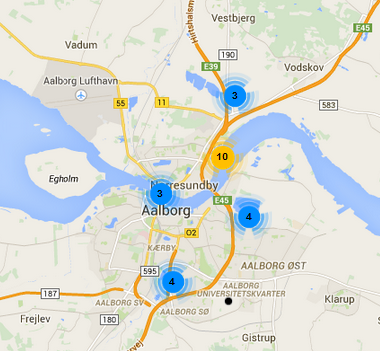
\includegraphics{MarkerClusterer}
\caption{A result of the MarkerClusterer library}
\label{fig:markerclusterer}
\end{center}
\end{figure}

\subsection{Usability Testing on Admin Part}
We had originally wanted to usability test both the public and administrative parts of the website.
Usability tests were performed on the public part, and problems were found and resolved. 
The administrative users were, however, not available for usability testing.
This usability could have given more features to be implemented on the admin page, which had not been thought of.
It could also have resolved potential problems that we were not previously aware of it.
Furthermore, the usability test would be sufficient to make sure that the admins could use the page.

The admin usability test should be done before the website is released, since it might reveal some problems with the page.

\subsection{Sending Unlock Code over SMS}
Originally, it had been intended that the unlock code for a booking would be sent over SMS. 
This seemed out of scope for the project and it would have cost money to do so, as such it was decided to provide the unlock code on the front page. 
This, however, is something that could be added in the future.
	\chapter{Conclusion}
	
	\afterpage{\thispagestyle{empty}}

	\bibliography{Bibliography}
	
	\label{lastpagewithoutappendix}

	\appendix
	\chapter{Website Architecture}

\section{Controllers}
\begin{figure}[h]
	\centering
	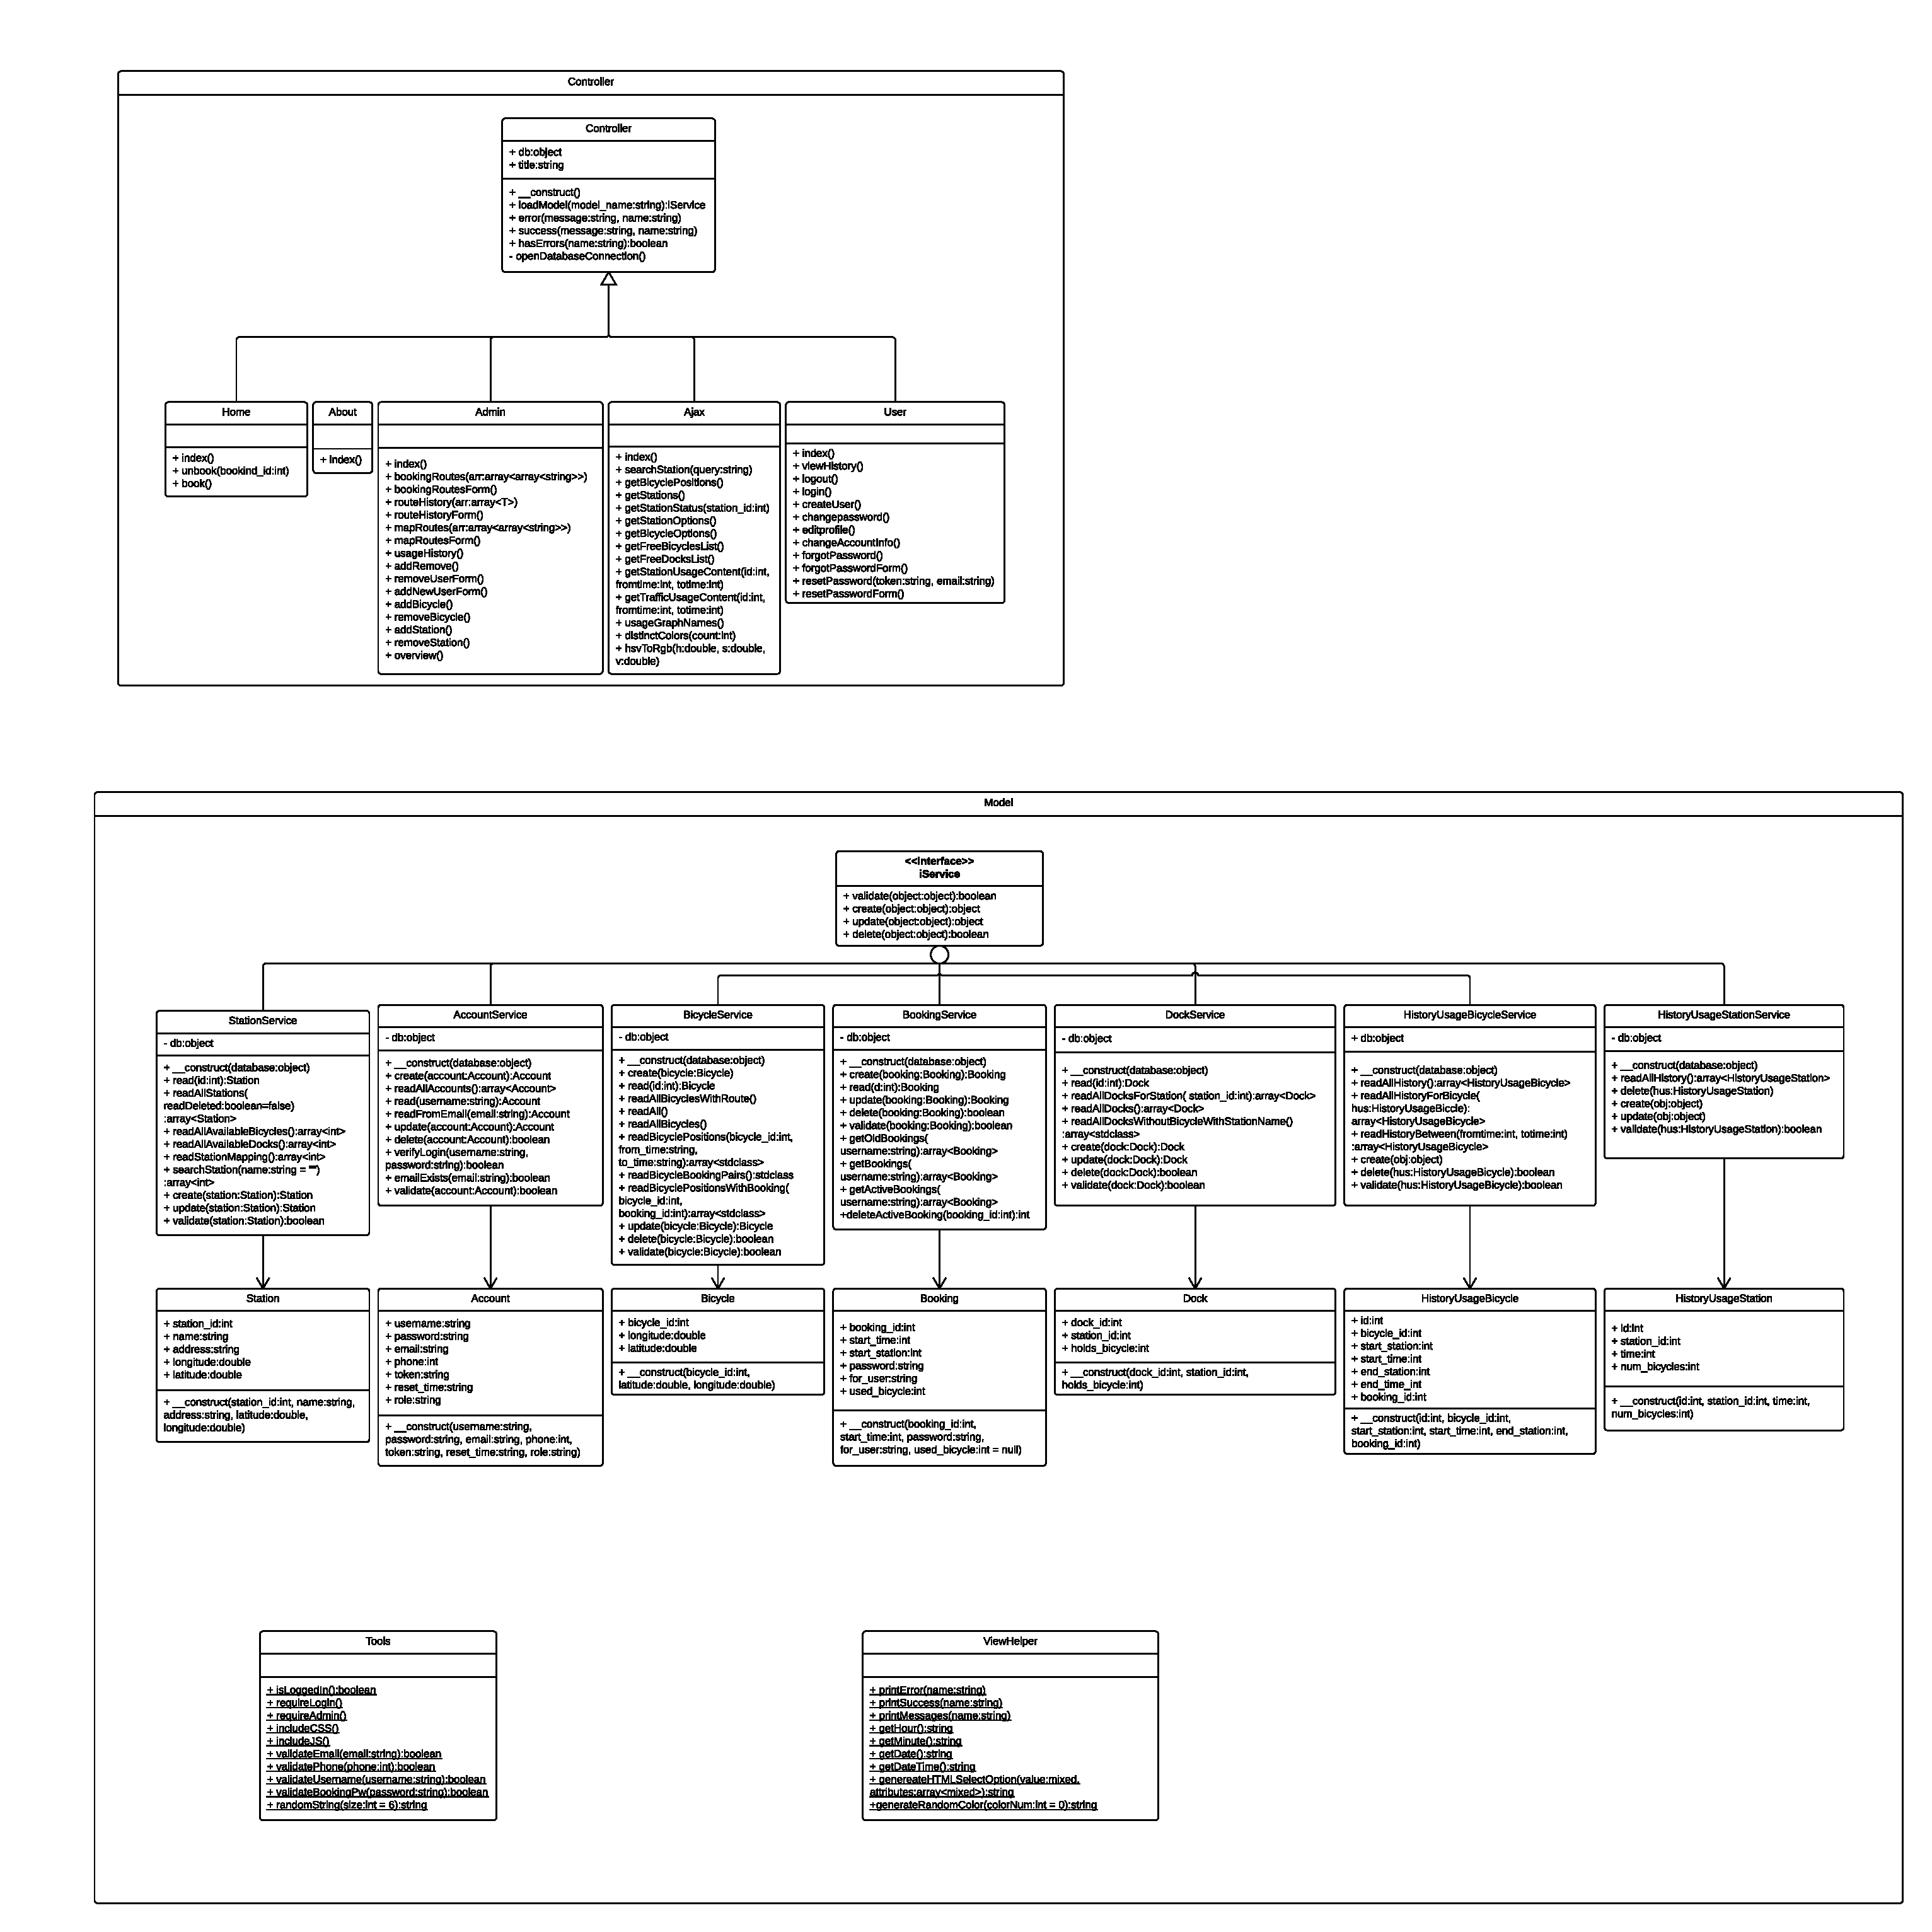
\includegraphics[scale=0.5, trim = 3cm 33cm 22cm 1cm,clip]{design/all-architecture}
\end{figure}
%l b r t

\newpage
\section{Model}

\begin{figure}[h]
	\centering
	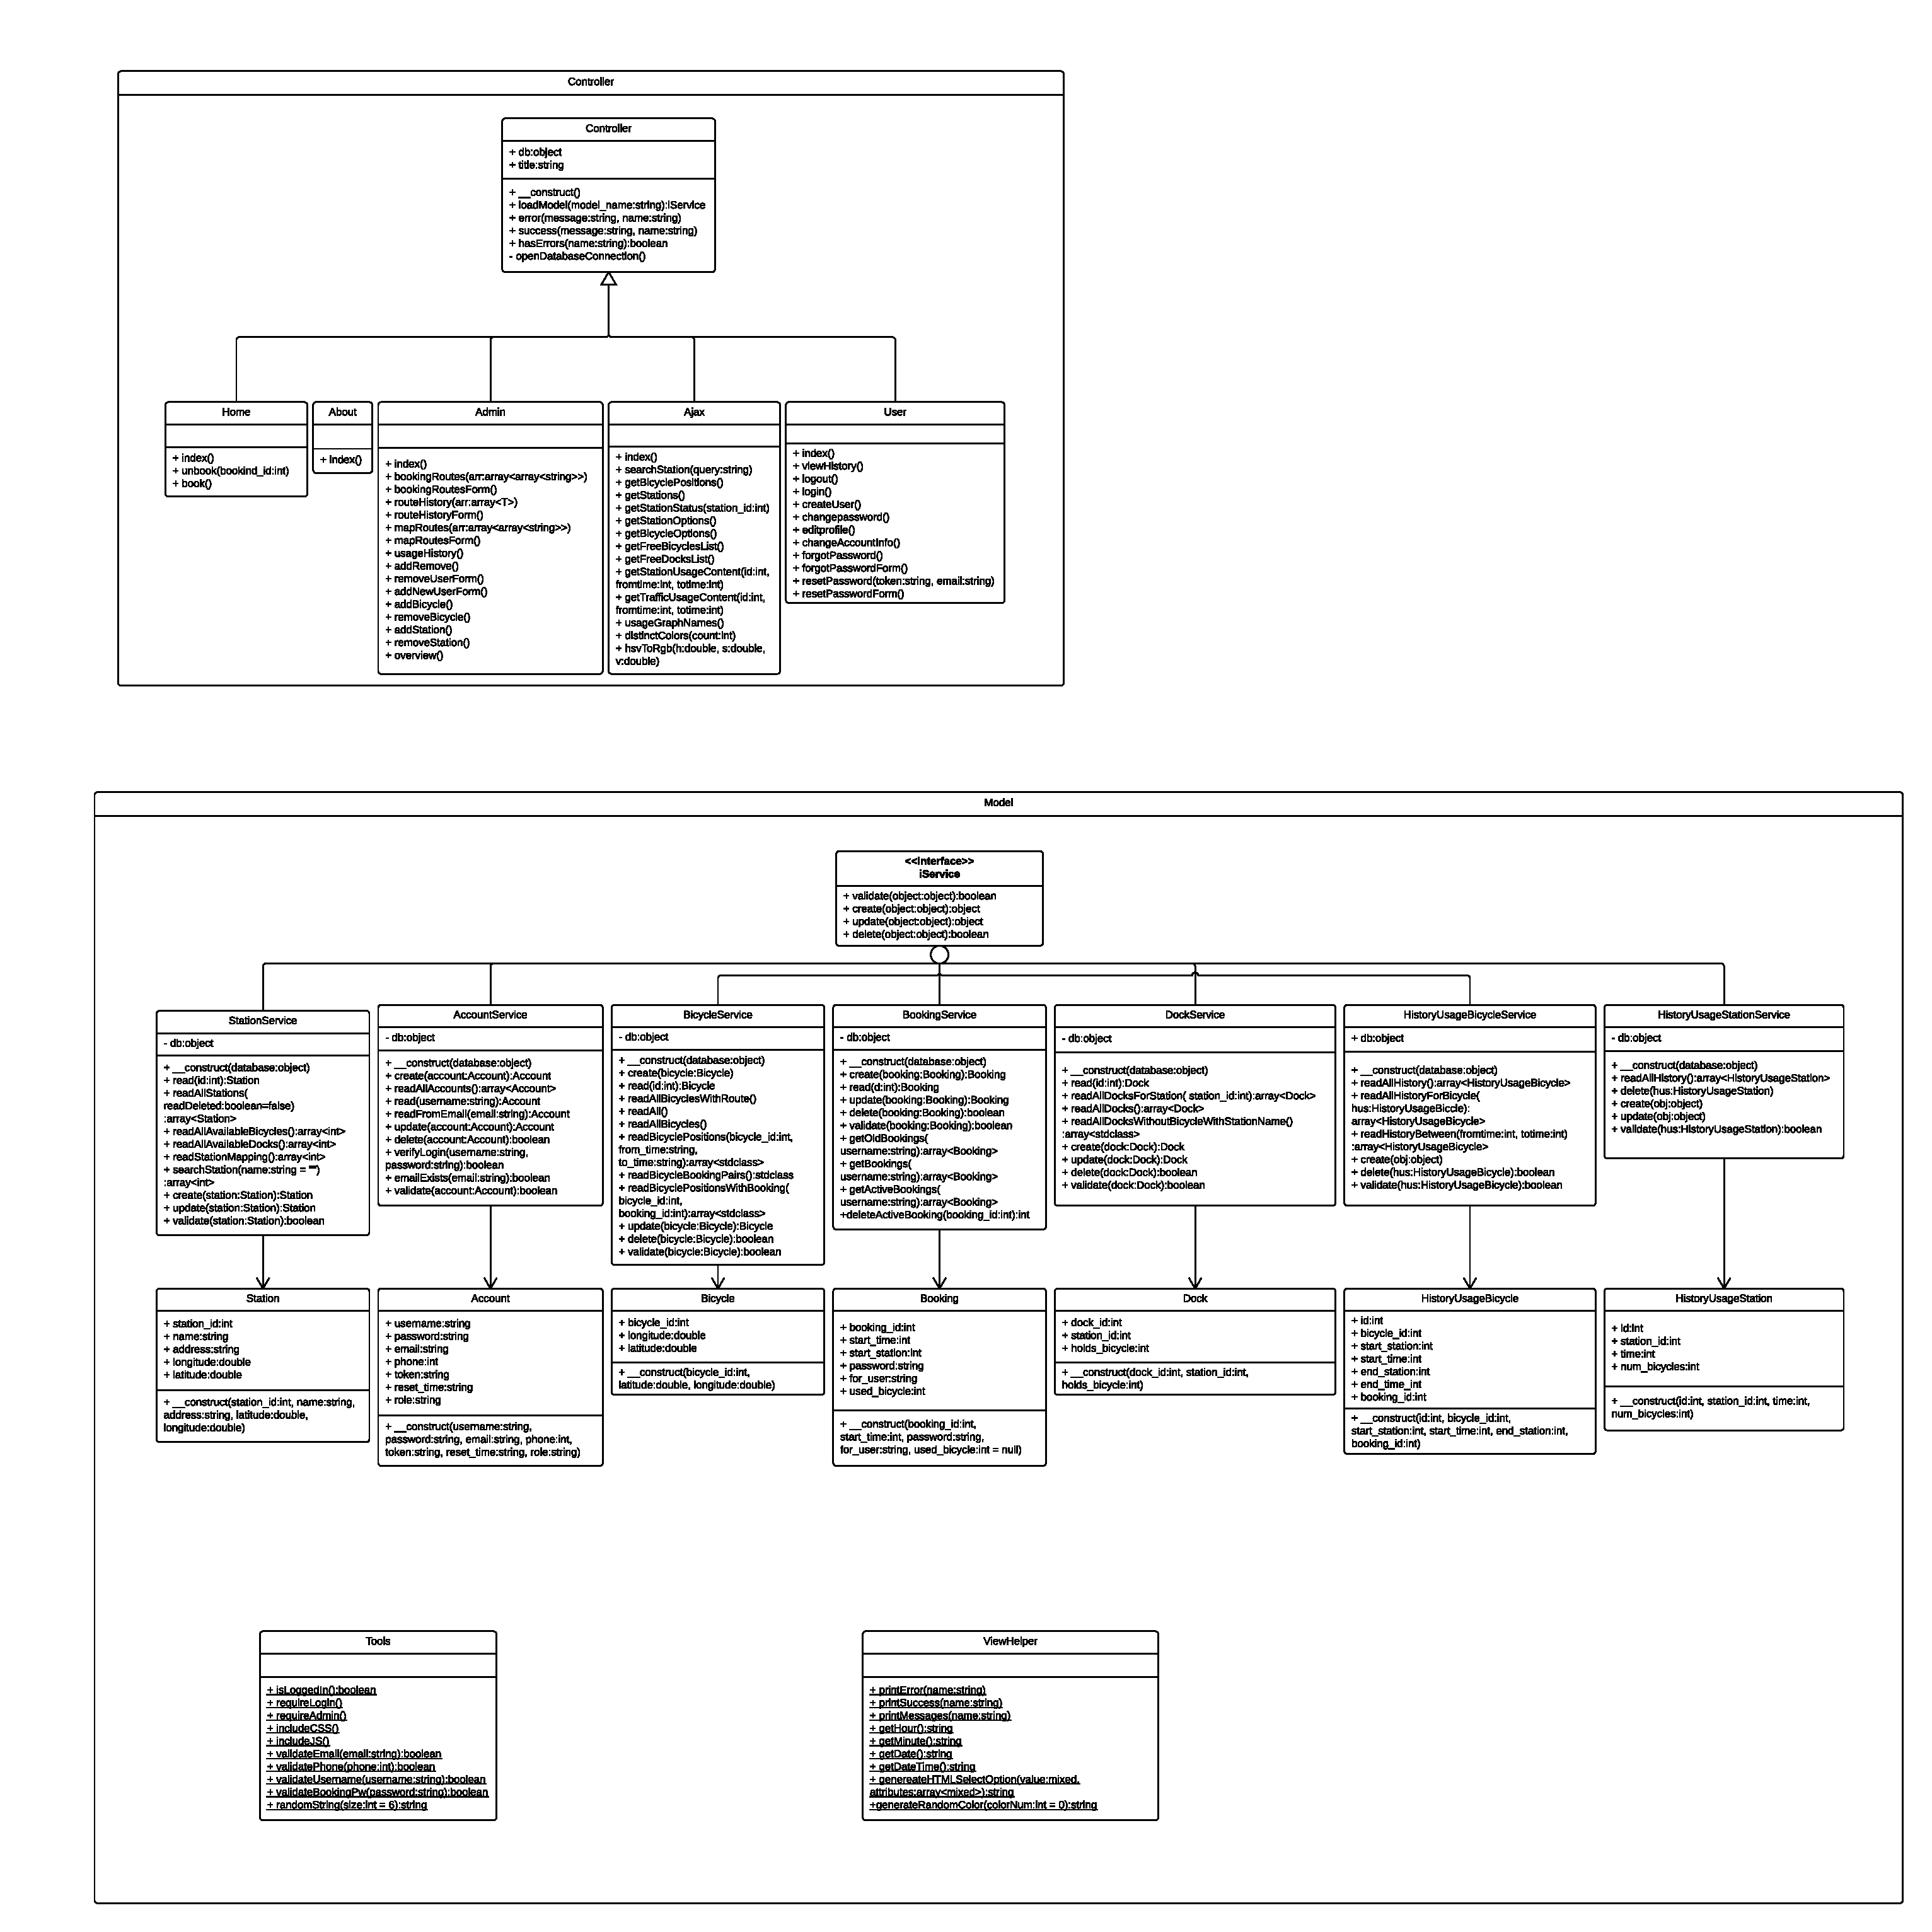
\includegraphics[scale=0.355, angle = -90, trim = 0cm 0cm 0.5cm 21cm,clip]{design/all-architecture}
\end{figure}
%l b r t
	\chapter{Admin Site}
\section{Add-Remove}\label{app:addremove}
\begin{figure}[h]
	\centering
	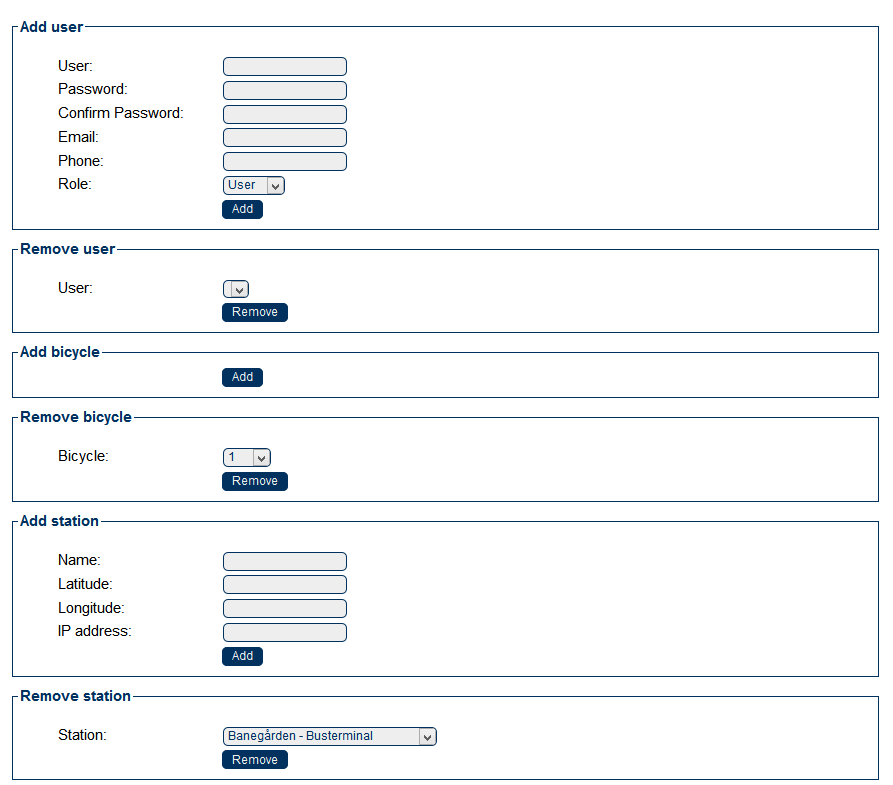
\includegraphics[scale=0.43, clip, trim = 0.25cm 0.75cm 0.25cm 2cm]{appendix/addRemove}
\end{figure}


	\documentclass[10pt,a4paper]{article}
\usepackage[latin1]{inputenc}
\usepackage{amsmath}
\usepackage{amsfonts}
\usepackage{amssymb}
\usepackage{graphicx}
\usepackage{enumitem}
\usepackage{enumerate}

\begin{document}
	\section*{Usability Test}
    Om usability testen g�lder det at du ikke skal v�re bange for at pr�ve dig frem, der sker ikke noget farligt hvis du laver en fejl.
    Derudover vil vi gerne have dig til at t�nke h�jt m.h.t. det du t�nker og foretager dig i testen.
    Du bedes venligst l�se en opgave h�jt f�r du udf�rer den.
    
	\subsection*{Hjemmeside Del}
    Siden du kommer til at pr�ve nu er en side der g�r det muligt at booke aalborg bycykler.
    Du vil komme gennem forskellige dele af hjemmesiden der har at g�re med booking og status for aalborg bycykler.
	
	\begin{description}[style=nextline]
		\item[Tag et kig p� siden]
			Tag dig god tid til at kigge lidt rundt p� siden, for at se hvordan siden er opbygget. 
		\item[Find status for cykel]
			Du overvejer at l�ne en bycykel fra Baneg�rden men er ikke sikker p� om der er flere ledige bycykler ved stationen.
			
			Find antal ledige cykler for stationen: "Baneg�rden Busterminal".
		\item[Booking - Login Del]
			For at f� adgang til at booke en cykel skal man v�re logget ind, du har heldigvis allerede en bruger med f�lgende login oplysninger:
			
			\textbf{Brugernavn:} testbruger
			
			\textbf{Adgangskode:} testkode
			
			Brug ovenst�ende loginoplysninger til at logge ind med.
		\item[Booking - v�lg tid og book del]
			 Du er nu logget ind og er klar til at booke en cykel.
			 
			 Book en cykel til i morgen kl. 11:25
		\item[Afmelding af planlagt booking]
			 Du kommer til at se at der er en anden booking, ogs� til i morgen men kl. 11:45 og ved Kunsten.
			 Denne booking er ikke n�dvendig og du vil gerne have den afmeldt.
			 
			 Afmeld bookingen der er til i morgen kl. 11:45 ved Kunsten.
		\item[Se booking historik]
			 Du har nu f�et booket en cykel til i morgen, og afmeldt en anden booking.
			 Dog vil du gerne se en historik over alle dine bookings, b�de dem der er tilmeldt og aflyste.
			 
			 Find og l�s booking-historikken for din profil.
	\end{description}
	
	\subsection*{Stations Del}
\end{document}
	\cleardoublepage
	\phantomsection
\end{document}
